\documentclass[10pt]{beamer}
\usetheme{Boadilla}
\usefonttheme{serif}

\usepackage[utf8]{inputenc}
\usepackage[UKenglish]{babel}
\usepackage[T1]{fontenc}
\usepackage{hyperref}
\usepackage{pgfgantt}
\usepackage{csquotes}
\usepackage{amsmath}
\usepackage{amsfonts}
\usepackage{xcolor}
\usepackage{amssymb}
\usepackage{graphicx}
\usepackage{subfigure}
\usepackage{lmodern}
\usepackage{float}
\usepackage{multicol}
\usepackage{hyperref}

\newcommand{\bib}[1]{$^\text{\cite{#1}}$}

\author{Steve de Rose}
\title{Morphotype of the human body}
\subtitle{a clustering approach}
\date{}

\begin{document}
\begin{frame}
	\bibliographystyle{ieeetr}
	\begin{figure}[H]
		\begin{minipage}{0.48\textwidth}
			\centering
			
\includegraphics[width=.5\linewidth]{../Images/Logo_UTT.png}
		\end{minipage}\hfill
		\begin{minipage}{0.48\textwidth}
			\centering
			
\includegraphics[width=.5\linewidth]{../Images/ifth_retina.png}
		\end{minipage}
	\end{figure}
	\maketitle

	\begin{center}
		\footnotesize
		\textit{Supervised by :}\\
		\href{mailto:frederic.bertrand@utt.fr}{Frédéric Bertrand (UTT)}\\
		\href{mailto:myriam.maumy@utt.fr}{Myriam Maumy Bertrand (UTT)}\\
		\href{mailto:philippe.meyer@utt.fr}{Philippe Meyer (UTT)}\\
	\end{center}
\end{frame}

\begin{frame}{Context: LabCom DiTex}
	DiTeX is a joint research and development laboratory between the University of Technology of Troyes and the French Institute of Textiles and Clothing.
	\vspace{5mm}

	\begin{block}{Statistical modelling and machine learning to analyse data from clothing and to respond to problems.}
		\begin{itemize}
			\item The measurements of the human body:
			      \begin{itemize}
				      \item What is the effect of ageing?
				      \item What are the types of morphologies?
			      \end{itemize}
		\end{itemize}
	\end{block}
\end{frame}

\begin{frame}{Issue: Morphotypes}
	\begin{block}{}
		\begin{minipage}[cl]{0.5\textwidth}
			\begin{flushleft}
				The \textbf{variety of human morphologies} is an important issue for the textile-apparel industry.

				\only<+>{\begin{exampleblock}{}Enables proper organisation of garment sizing systems.\end{exampleblock}}
				\only<+->{\begin{exampleblock}{}
						How can these groups be defined?

						How do we associate an individual with a group?
					\end{exampleblock}}

			\end{flushleft}
		\end{minipage}%
		\begin{minipage}[H]{0.5\textwidth}
			\centering
			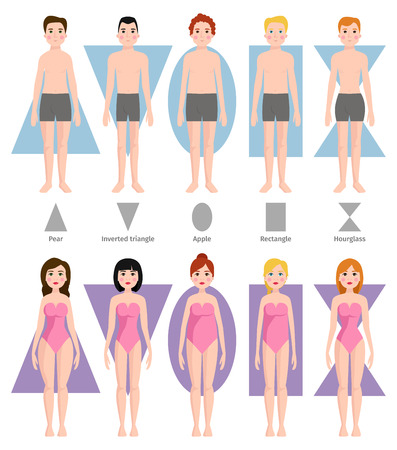
\includegraphics[width=0.85\textwidth]{../Images/Morph1.jpg}
		\end{minipage}
	\end{block}
\end{frame}

\section{State of the Art}
\begin{frame}{Early studies}
	\begin{block}{3rd century BC}
		Hippocrates\bib{Croney} recorded two distinct shapes of the human body:
		\begin{itemize}
			\item thin/tall
			\item short/thick
		\end{itemize} \pause
	\end{block}\pause
	\begin{block}{1940s}
		W. Sheldon\bib{Sheldon} defined the somatotype as the arrangement of three poles:
		\begin{itemize}
			\item endomorph
			\item mesomorph
			\item ectomorph
		\end{itemize}
	\end{block}
\end{frame}

\begin{frame}{Women's measurements for garments and pattern construction}
	\begin{block}{1941}
		O’Brien and Shelton study of women’s measurements\bib{ROB} :
		\begin{itemize}
			\item linear body measurement data of 14,698 women,
			\item statistical analysis.
		\end{itemize}\pause
		The analysis showed that girth measurements have little relation to vertical measurements.
	\end{block}
\end{frame}

\begin{frame}{20th century}
	\begin{block}{1968}
		Douty and Brannon\bib{Douty} used silhouette photographs to study body build and posture.
	\end{block}\pause
	\begin{block}{1978}
		Minott categorised female human body shapes in components\bib{Minott}.
	\end{block}\pause
	\begin{block}{1981} August\bib{Bonnie} categorised body shapes based on landmark identification and recognition by component.
	\end{block}\pause
	\begin{block}{1987}
		Armstrong\bib{Armstrong} described four female body shapes based on the shoulder/hip relationship.
	\end{block}
\end{frame}

\begin{frame}{Female Figure Identification Technique for apparel measurements}
	\begin{block}{2004}
		Simmons, Istook, and Devarajan developed a software\bib{FFIT1, FFIT2} to classify 3D body scans and identify body shapes. They used a sample of 887 subjects to validate the nine identified body shapes.
	\end{block}
	\vspace{4mm}
	\begin{exampleblock}{\centering\itshape Body shapes}
		\begin{multicols}{3}
			\begin{itemize}
				\item Hourglass	\item Bottom Hourglass	\item Top Hourglass
				\item Spoon		\item Triangle			\item Inverted Triangle
				\item Rectangle	\item Diamond			\item Oval
			\end{itemize}
		\end{multicols}
	\end{exampleblock}
\end{frame}

\begin{frame}{Comparison of body shape between USA and Korean women}
	\begin{block}{2007}
		Lee, Istook, Nam, and Park\bib{IJCST} used a mathematical analysis and visual inspection to develop formulas based on the descriptions of the original FFIT software categories.
	\end{block}

	\vspace{4mm}
	\begin{exampleblock}{\centering\itshape Formulas}
		\vspace{2mm}
		\begin{table}[H]
			\centering
			\textsf{\tiny
				\begin{tabular}{|l|l|}
					\hline
					\textbf{BODY TYPE} & {\textbf{MEASUREMENT}}                                                                                 \\
					\hline
					Hourglass          & (bust-hip)$\leqslant 25$), (hip-bust)$< 91$, (bust-waist)$\geqslant 230$ or (hip-waist)$\geqslant 250$ \\
					\hline
					Bottom hourglass   & (hip-bust)$\geqslant 91$ and (hip-bust)$< 250$, (bust-waist)$\geqslant 230$, (high hip/waist)$< 1.193$ \\
					\hline
					Top hourglass      & (bust-hip)$> 25$ and (bust-hip)$< 250$, (bust-waist)$\geqslant 230$                                    \\
					\hline
					Spoon              & (hip-bust)$> 51$, (hip-waist)$\geqslant 180$, (high hip/waist)$\geqslant 1.193$                        \\
					\hline
					Triangle           & (hip-bust)$\geqslant 91$, (hip-waist)$< 230$                                                           \\
					\hline
					Inverted Triangle  & (bust-hip)$\geqslant 91$, (bust-waist)$< 230$                                                          \\
					\hline
					Rectangle          & (hip-bust)$< 91$ and (bust-hip)$< 91$, (bust-waist)$\geqslant 230$ and (hips-waist)$< 250$             \\
					\hline
				\end{tabular}}
		\end{table}
	\end{exampleblock}
\end{frame}

\begin{frame}{Modification of the FFIT Formulas to Include Plus Size Bodies}
	\begin{block}{2020}
		Sokolowski and Bettencourt modified the FFIT mathematical formulas to be more inclusive of plus size women\bib{SSCB}.
	\end{block}
	\begin{exampleblock}{\centering\itshape Formulas}
		\vspace{2mm}
		\begin{table}[H]
			\centering
			\textsf{\tiny
				\begin{tabular}{|l|l|}
					\hline
					\textbf{BODY TYPE} & {\textbf{MEASUREMENT}}                                                                                       \\
					\hline
					Hourglass          & (bust-hip)$\leqslant 25$, (hip-bust)$< 91$, (bust-waist)$\geqslant 230$ or (hip-waist)$\geqslant 250$        \\
					\hline
					Bottom Hourglass   & (hip-bust)$\geqslant 91$ and (hip-bust)$< 250$, (hip-waist)$\geqslant 230$, (high hip/waist)$< 1.193$        \\
					\hline
					Top Hourglass      & (bust-hip)$> 1$ and (bust-hip)$< 250$, (bust-waist)$\geqslant 230$                                           \\
					\hline
					Spoon              & (hip-bust)$> 51$, (hip-waist)$\geqslant 178$, (high hip/waist)$\geqslant 1.193$                              \\
					\hline
					Triangle           & (hip-bust)$\geqslant 91$, $0 \leqslant$(hip-waist)$< 230$ or (bust-waist)$< 0$, (hip-waist)$\geqslant 0$     \\
					\hline
					Inverted Triangle  & (bust-hip)$\geqslant 91$, (bust-waist)$< 9$, (hip-waist)$\geqslant 0$                                        \\
					\hline
					Rectangle          & (hip-bust)$< 91$, and (bust-hip)$< 91$, $0 \leqslant$(bust-waist)$< 230$ and $0 \leqslant$(hip-waist)$< 250$ \\
					\hline
					Diamond            & (hip-waist)$< 0$, and (bust-waist)$< 0$                                                                      \\
					\hline
					Oval               & (hip-waist)$< 0$, and (bust-waist)$\geqslant 0$                                                              \\
					\hline
				\end{tabular}}
		\end{table}
	\end{exampleblock}
\end{frame}

\begin{frame}{Body Shape Assessment Scale}
	\begin{block}{2006}
		Connell, Ulrich, Brannon, Alexander and Presley developed a series of scales to assess women's body shapes as seen on body scanners\bib{BSAS}.

		From 42 body scans of women aged 20 to 55, they developed nine scales based on frontal and lateral views.\pause
		\begin{itemize}
			\item 3 (Body Build, Body Shape, Posture) were for whole body analysis,\pause
			\item 6 (Front Torso Shape, Hip Shape, Shoulder Slope, Chest Shape, Buttock Shape, Back Curvature) for body part analysis.
		\end{itemize}
	\end{block}
\end{frame}

\begin{frame}{Analysis and classification of 3D trunk shape}
	\begin{block}{2009}
		Nakamura and Kurokawa used the 3D measurements of 560 Japanese women aged 19 to 63 years taken in laser metrology.
		\begin{itemize}
			\item data obtained for each subject consisted of approximately 160,000 body surface points.
			\item after shape data reduction, $111$ representative coordinates that can cover approximately $92\%$ of the original coordinates were chosen as the dataset for shape analysis.
		\end{itemize}
		Then, they applied principal component analysis with varimax rotation.
	\end{block}
\end{frame}

\begin{frame}{Analysis and classification of 3D trunk shape}
	\begin{block}{Data analysis}
		Nakamura and Kurokawa then performed cluster analysis of the scores of the six principal components.
		\begin{itemize}
			\item They adopted Ward's method\bib{Ward} and used the squared Euclidean distance as the metric.
			\item The component scores are not normalized.
			\item Based on the dendrogram, they judged that 'five' is an appropriate number of classes.
		\end{itemize}
		Therefore, they obtained five classes: C1, C2, C3, C4 and C5.
	\end{block}
\end{frame}

\begin{frame}{Analysis and classification of 3D trunk shape}
	\begin{figure}[H]
		\centering
		\caption{\small\centering\itshape Dendrogram of cluster analysis and the level of the five classes}
		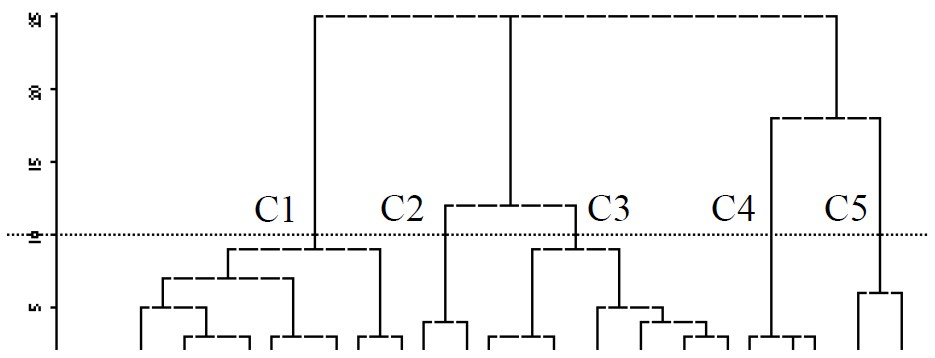
\includegraphics[width=0.9\linewidth]{../Images/Kuro2.jpg}
	\end{figure}
\end{frame}

\begin{frame}{Analysis and classification of 3D trunk shape}
	\begin{figure}[H]
		\caption{Average figures in the classes C1 to C5}
		\centering
		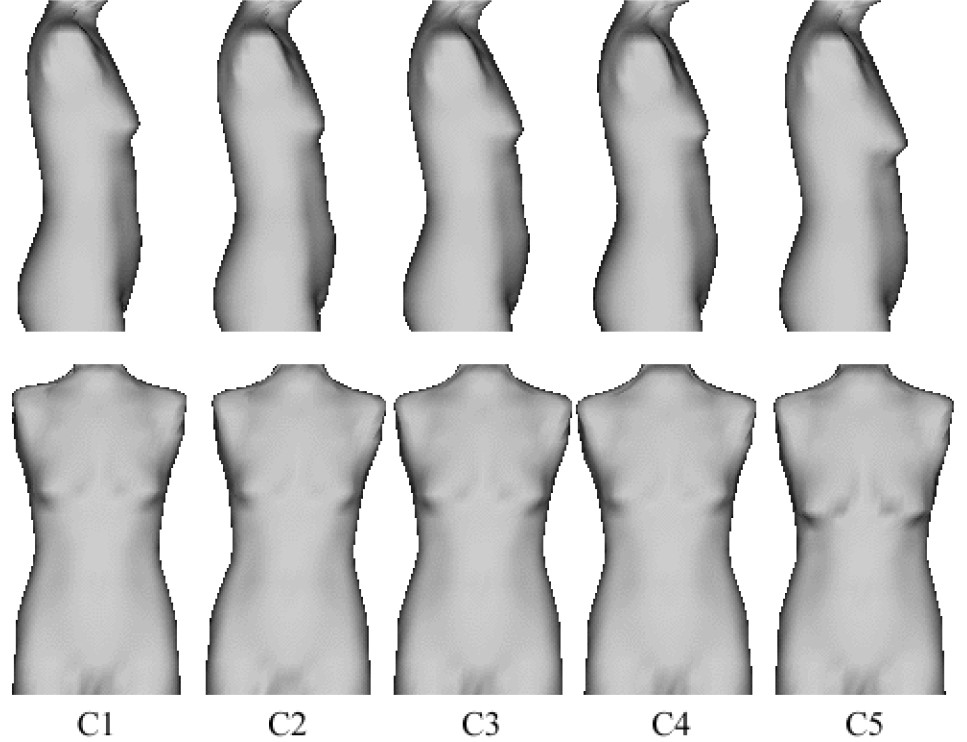
\includegraphics[width=0.6\linewidth]{../Images/Kuro3.jpg}
	\end{figure}
\end{frame}

\begin{frame}{Statistical human body form classification: Methodology development and application}
	\begin{block}{2012}
		Cottle\bib{phdthesis} developed a methodology to explore body shape analysis using 3D digital data generated by the body scanner.

		The methodological framework is an adaptation of Costa and Cesar's framework for computational pattern analysis:
		\begin{enumerate}
			\item Form preprocessing
			\item Form transformations
			\item Form classification
		\end{enumerate}
	\end{block}
\end{frame}

\begin{frame}
	\begin{block}{Data analysis}
		\begin{itemize}
			\item 117 body scan files were used from the Men’s Mentoring Study\bib{MMS}.
			\item PCA to reduce the number of data points from $32,000$ to $3,104$.
			\item Unsupervised classification or clustering used to develop a hierarchical clustering of subjects.
		\end{itemize}
	\end{block}
	\begin{exampleblock}{Clustering of male body form}
		Applying the clustering technique established in the pretest to the $3\,104$ variables (height, weight, and 3D body scan data), seven distinct body form clusters emerged.

		\begin{center}
			{\scriptsize
				\begin{tabular}{cccccc}
					\hline
					Cluster & number & Age (years) & Weight (kg) & Height (cm) & BMI   \\
					\hline
					1       & 38     & 23.55       & 69.12       & 176.32      & 22.34 \\
					2       & 3      & 25.67       & 72.27       & 182.88      & 21.67 \\
					3       & 45     & 24.38       & 81.65       & 179.60      & 25.36 \\
					4       & 5      & 24.80       & 80.65       & 177.80      & 25.60 \\
					5       & 15     & 27.00       & 96.65       & 182.70      & 29.20 \\
					6       & 5      & 27.80       & 112.85      & 187.45      & 32.20 \\
					7       & 6      & 29.33       & 135.40      & 182.88      & 40.83 \\
					\hline
				\end{tabular}}
		\end{center}
	\end{exampleblock}
\end{frame}

\begin{frame}{Body shape analyses of large persons in South Korea}
	\begin{block}{2013}
		Park and Park studied the body shapes of large people using anthropometric data from South Korea.\bib{ERGO}
		\begin{itemize}
			\item A total of $1\,444$ males and $1\,327$ females were identified from the SizeKorea database.
			\item A total of 33 and 36 body dimensions were selected for males and females, respectively.
			\item For each gender, a factor analysis was conducted on the corresponding anthropometric data set. The varimax orthogonal rotation method\bib{Hair} was used.
			\item Ward's method was performed for each gender.
		\end{itemize}
	\end{block}
\end{frame}

\begin{frame}{Body shape analyses of large persons in South Korea}
	\begin{minipage}{0.45\textwidth}
		\centering
		\begin{block}{Male dataset results}
			Five factors were identified, which collectively accounted for $81.53\%$ of the total variance.
		\end{block}
		\begin{figure}[H]
			\centering
			\caption{\footnotesize\centering\itshape Korean males.}
			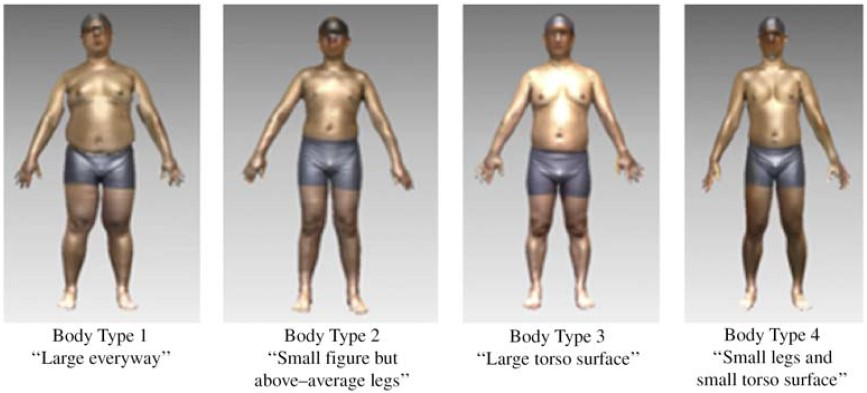
\includegraphics[width=\textwidth]{../Images/Park1}
		\end{figure}
	\end{minipage}\hfill
	\begin{minipage}{0.45\textwidth}
		\centering
		\begin{block}{Female dataset results}
			Three factors were identified, which collectively accounted for 74.10\% of the total variance.
		\end{block}
		\begin{figure}[H]
			\centering
			\caption{\footnotesize\centering\itshape Korean females.}
			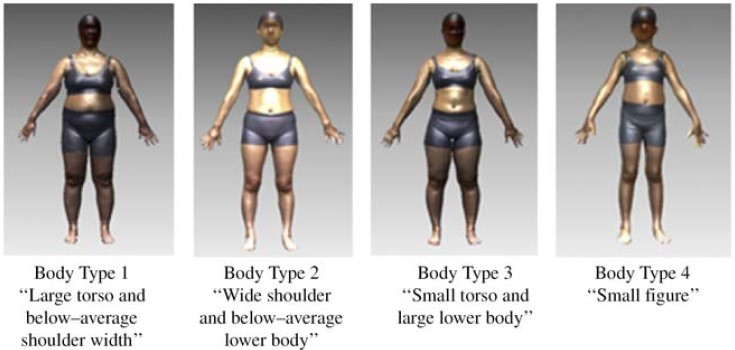
\includegraphics[width=\textwidth]{../Images/Park2}
		\end{figure}
	\end{minipage}
\end{frame}

\section{Human body form classification}
\subsection{Clustering methods}
\begin{frame}{K-Medoids algorithm}
	\begin{block}{PAM}
		A medoid is the most central representative of a class.

		It minimises the distance between the points of the class and the medoid.

		The PAM\bib{PAM} algorithm is based on finding k medoids among the observations in the dataset.
		\begin{itemize}
			\item After finding a set of k medoids, clusters are constructed by assigning each observation to the closest medoid.
			\item If the sum of dissimilarities of all objects with their closest medoid can be reduced by swapping a selected object (medoid) with a non-selected object, then a swap is performed.
			\item This is continued until the sum of dissimilarities cannot be reduced any further.
		\end{itemize}
	\end{block}
\end{frame}

\begin{frame}{Hierarchical clustering algorithm}
	\begin{block}{Ward's Method}
		Ward\bib{Ward}'s minimum variance criterion minimises the total variance within clusters.

		At each step, the pair of clusters that results in a minimum increase in total variance within the cluster after merging must be found.

		The Euclidean distance between the factor score vectors of two individuals was used as a measure of dissimilarity.
	\end{block}
\end{frame}

\begin{frame}{Finding the optimal number of clusters}
	\begin{block}{Number of clusters}
		For the same dataset, there are many possible partitionings\bib{KSel}.
		It is therefore necessary to choose the most relevant number of clusters K to highlight the interesting patterns.
		Unfortunately, there is no automatic procedure for this.
	\end{block}\pause
	\begin{exampleblock}{Choice of the method}
		Most of the indices account for both the separation and the compactness of clusters.\bib{KSel}

		Therefore, we will use the elbow method.
	\end{exampleblock}
\end{frame}

\begin{frame}{Finding the optimal number of clusters}
	\begin{block}{Elbow method}
		Empirical method that consists of running the clustering algorithm with different K values, calculating the variance between the clusters, and then placing the different numbers of K clusters according to the variance on a graph.
	\end{block}
	\begin{figure}[H]
		\centering
		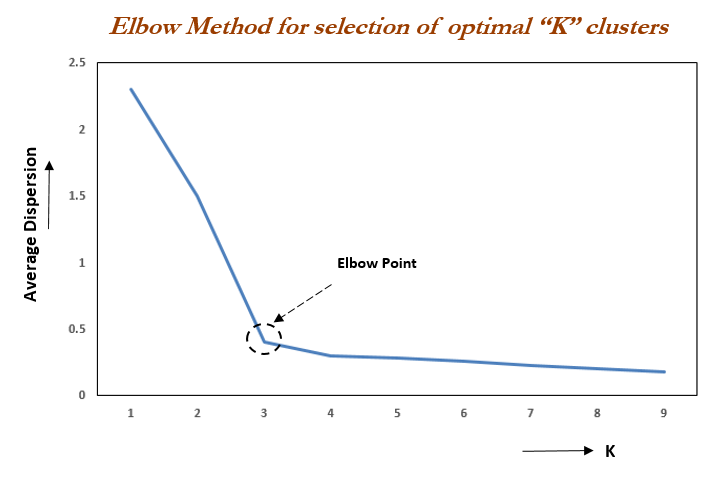
\includegraphics[width=0.5\textwidth]{../Images/Elbow_Method.png}\bib{Elbow}
	\end{figure}
\end{frame}

\subsection{Data sets}
\begin{frame}{Database}
	\begin{block}{ANSUR II}
		Data from the Anthropometric Survey of U.S. Army Personnel\bib{ANSUR}
		\begin{itemize}
			\item published internally in 2012
			\item made available to the public in 2017
			\item include 93 measurements for over 6,000 US military adults
			      \begin{itemize}
				      \item 4,082 men
				      \item 1,986 women
			      \end{itemize}
		\end{itemize}
	\end{block}
\end{frame}

\begin{frame}{Data sets preparation}
	\begin{block}{Data selection}
		We decide to keep only 14 torso and thigh measurements.
	\end{block}
	\begin{exampleblock}{\centering\itshape Measurements}
		\begin{multicols}{2}
			\begin{itemize}
				\item bicristal breadth
				\item buttock circumference
				\item buttock depth
				\item chest breadth
				\item chest circumference
				\item chest depth
				\item hip breadth
				\item lower thigh circumference
				\item shoulder circumference
				\item thigh circumference
				\item vertical trunk circumference
				\item waist breadth
				\item waist circumference
				\item waist depth.
			\end{itemize}
		\end{multicols}
	\end{exampleblock}
\end{frame}

\subsection{Female Data Set}
\begin{frame}{Results}
	We present the results we have obtained but, due to time constraints, we have not had time to discuss them.
	\begin{block}{Female data set}
		\centering
		\begin{tabular}{|cccc|c|}
			\hline
			Age   & Height (cm) & Weight (kg) & BMI   & \textit{Count} \\
			\hline
			28.94 & 164.09      & 66.91       & 24.82 & \textit{1986}  \\
			\hline
		\end{tabular}
	\end{block}
\end{frame}

\begin{frame}{Correlation matrix}
	\centering
	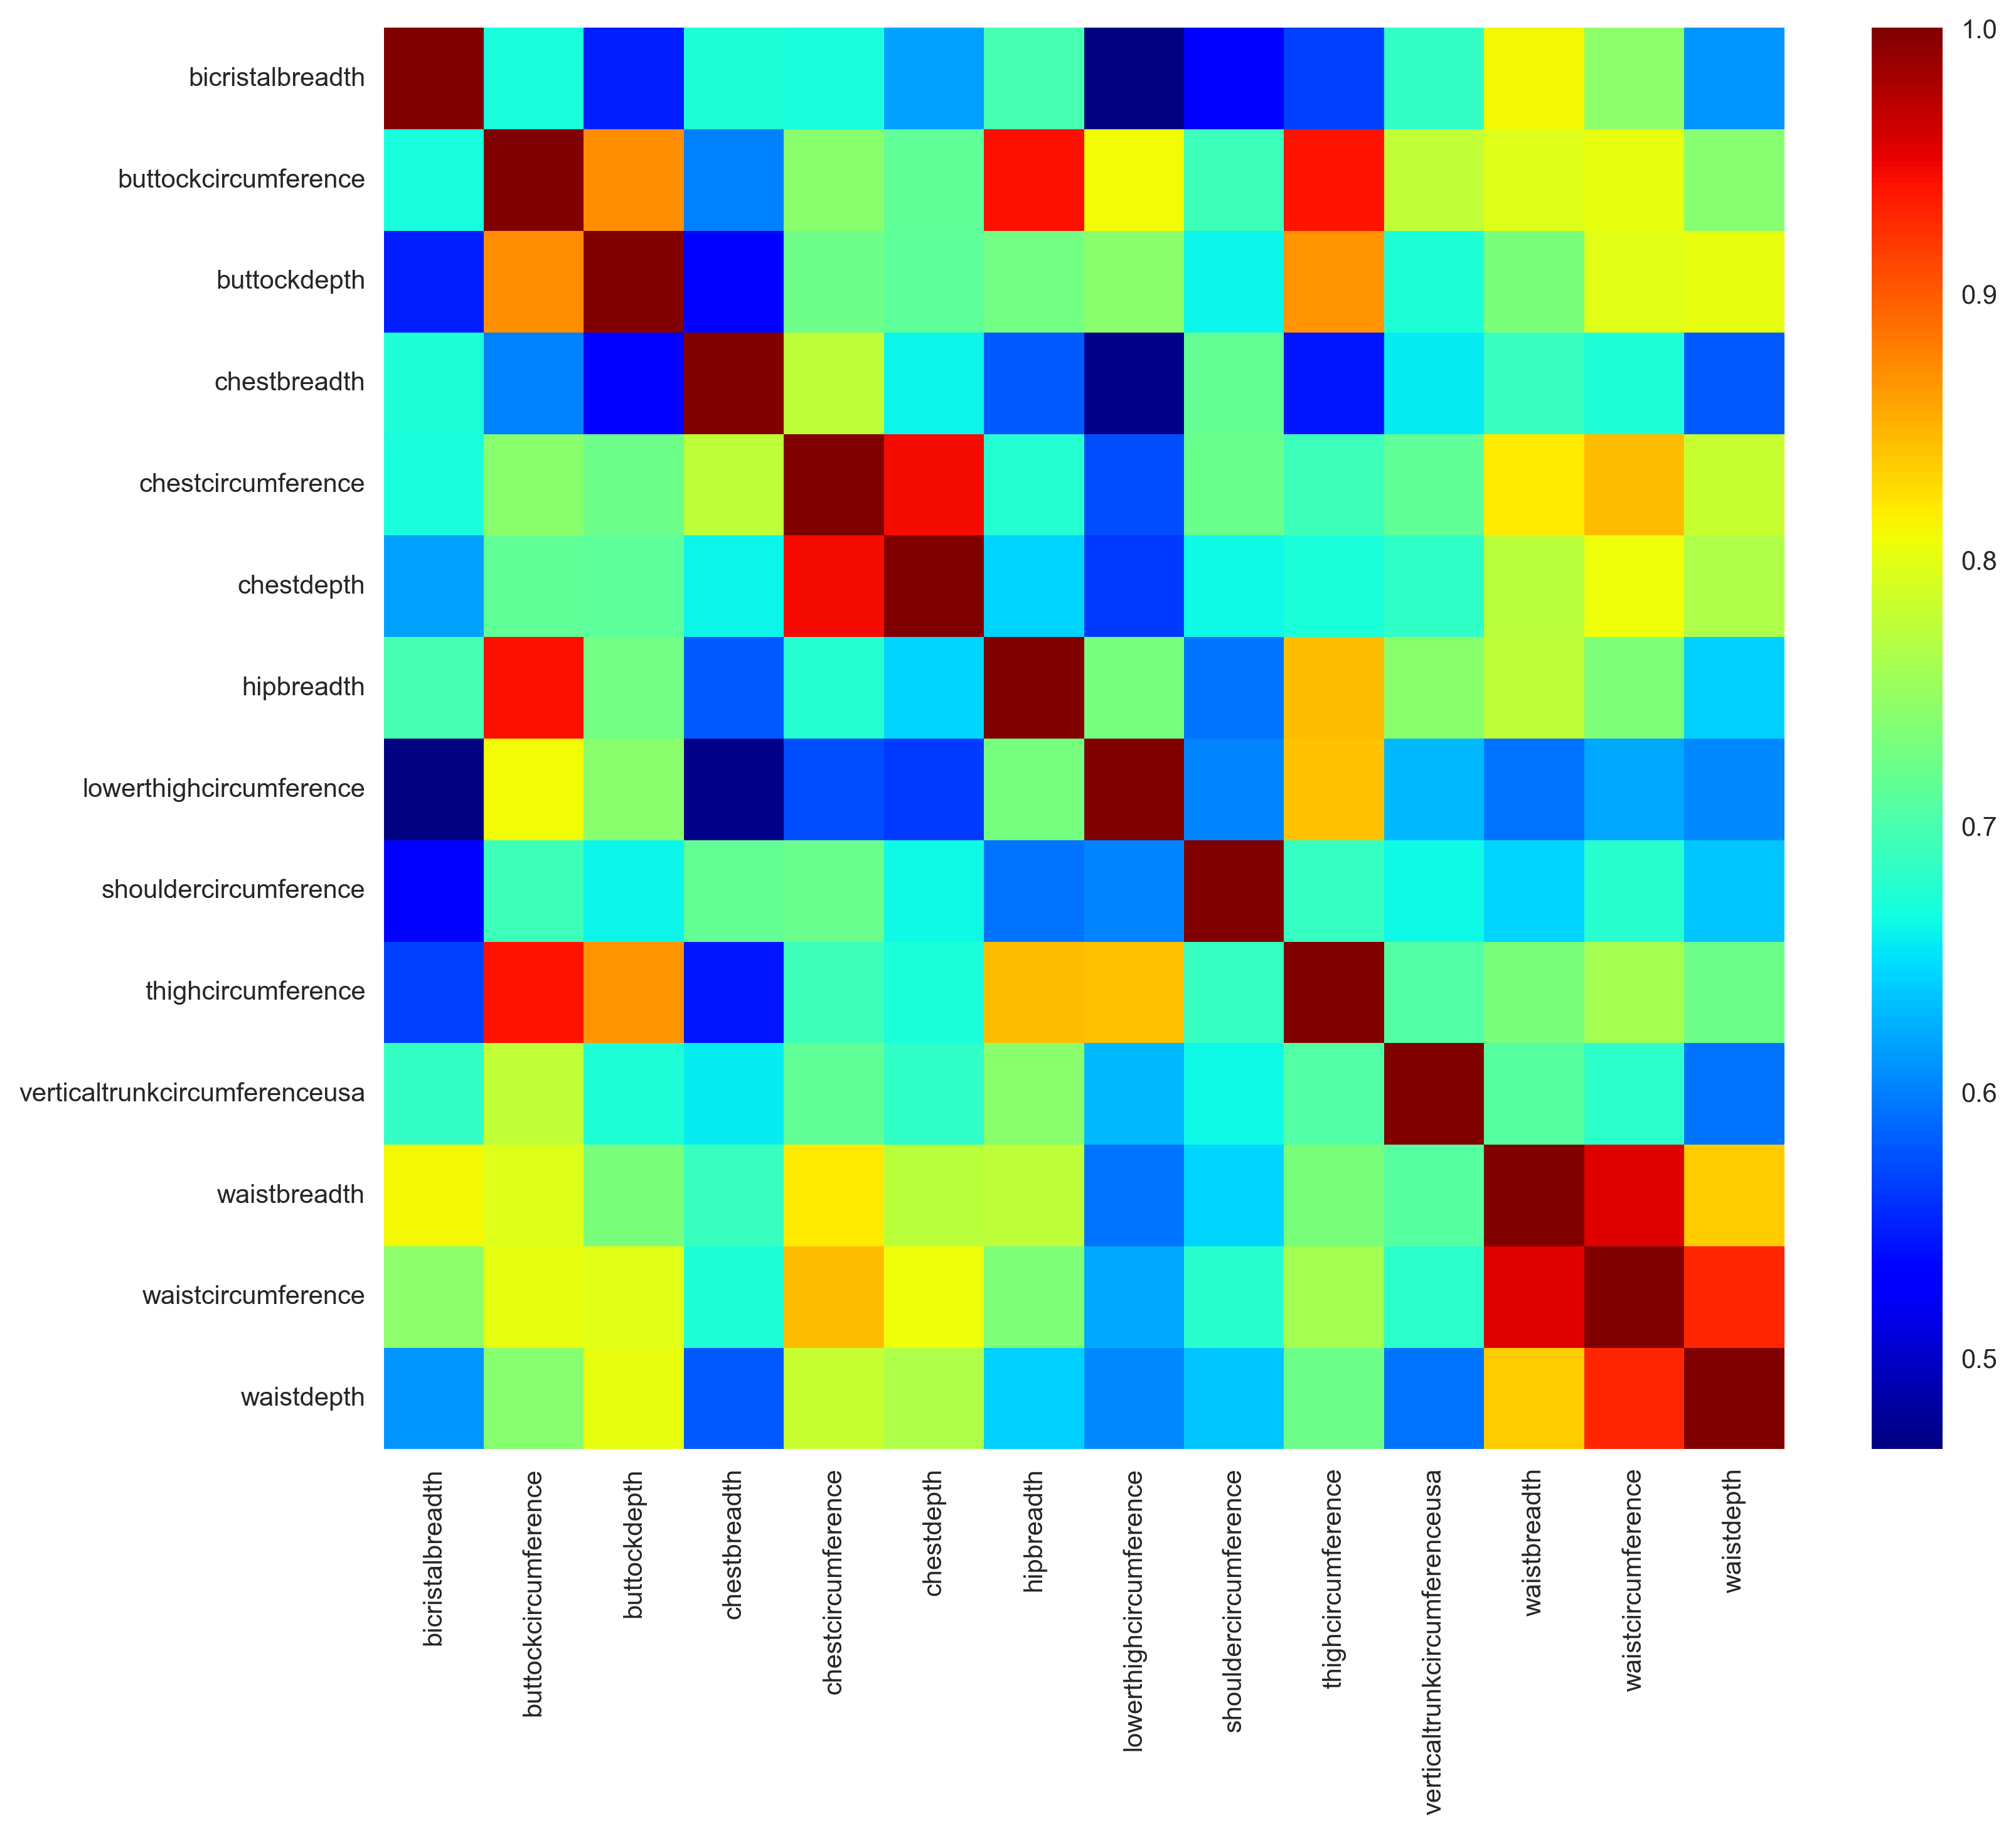
\includegraphics[width=0.7\textwidth]{../Images/FCorr.png}
\end{frame}

\begin{frame}{Elbow method}
	\subsubsection{K-Medoids}
	\begin{minipage}{0.55\textwidth}
		\centering
		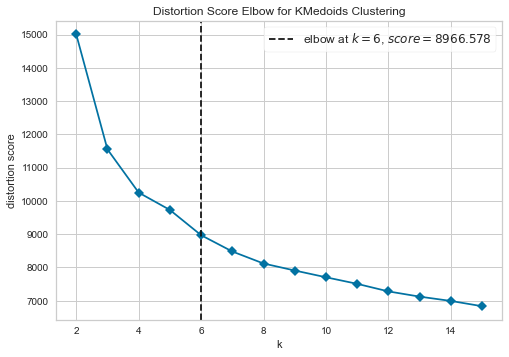
\includegraphics[width=0.8\textwidth]{../Images/FMedoidsElbow.png}
	\end{minipage}
	\begin{minipage}{0.3\textwidth}
		\itshape\scriptsize
		We choose a number of clusters $k=6$ for the K-Medoids.
	\end{minipage}
	\begin{minipage}{0.55\textwidth}
		\centering
		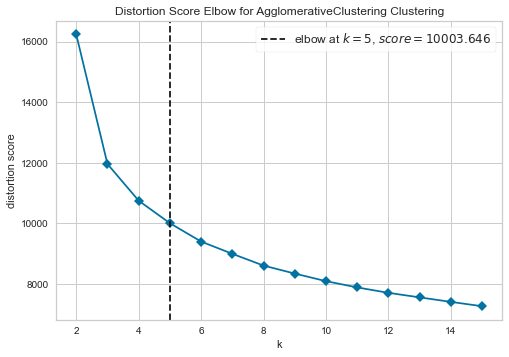
\includegraphics[width=0.8\textwidth]{../Images/FHierElbow.png}
	\end{minipage}
	\begin{minipage}{0.3\textwidth}
		\itshape\scriptsize
		We choose a number of clusters $k=5$ for the Ward's method.
	\end{minipage}
\end{frame}
\subsubsection{Visualisation}
\begin{frame}{K-Medoids Clusters}
	\centering
	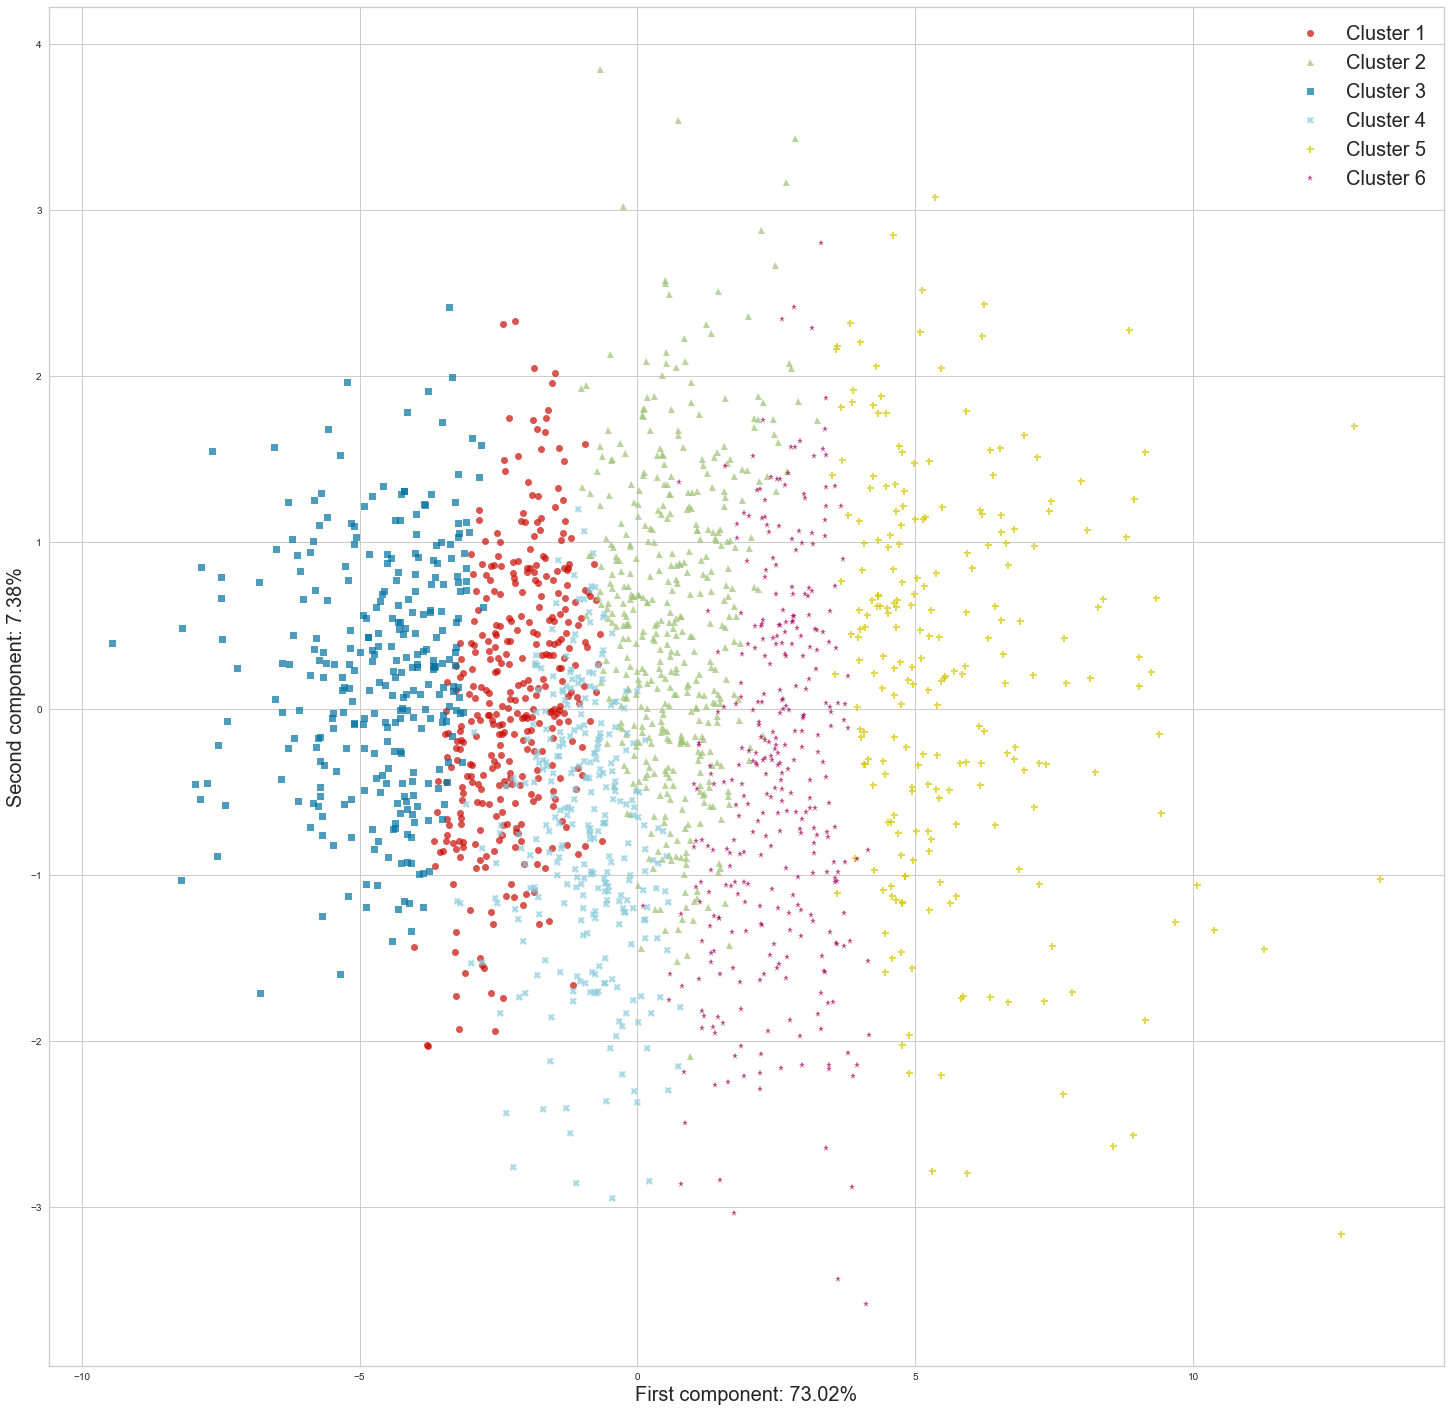
\includegraphics[width=0.675\textwidth]{../Images/FMedoidsProjection.png}
\end{frame}

\begin{frame}{Female Ward's Method Dendrogram}
	\centering
	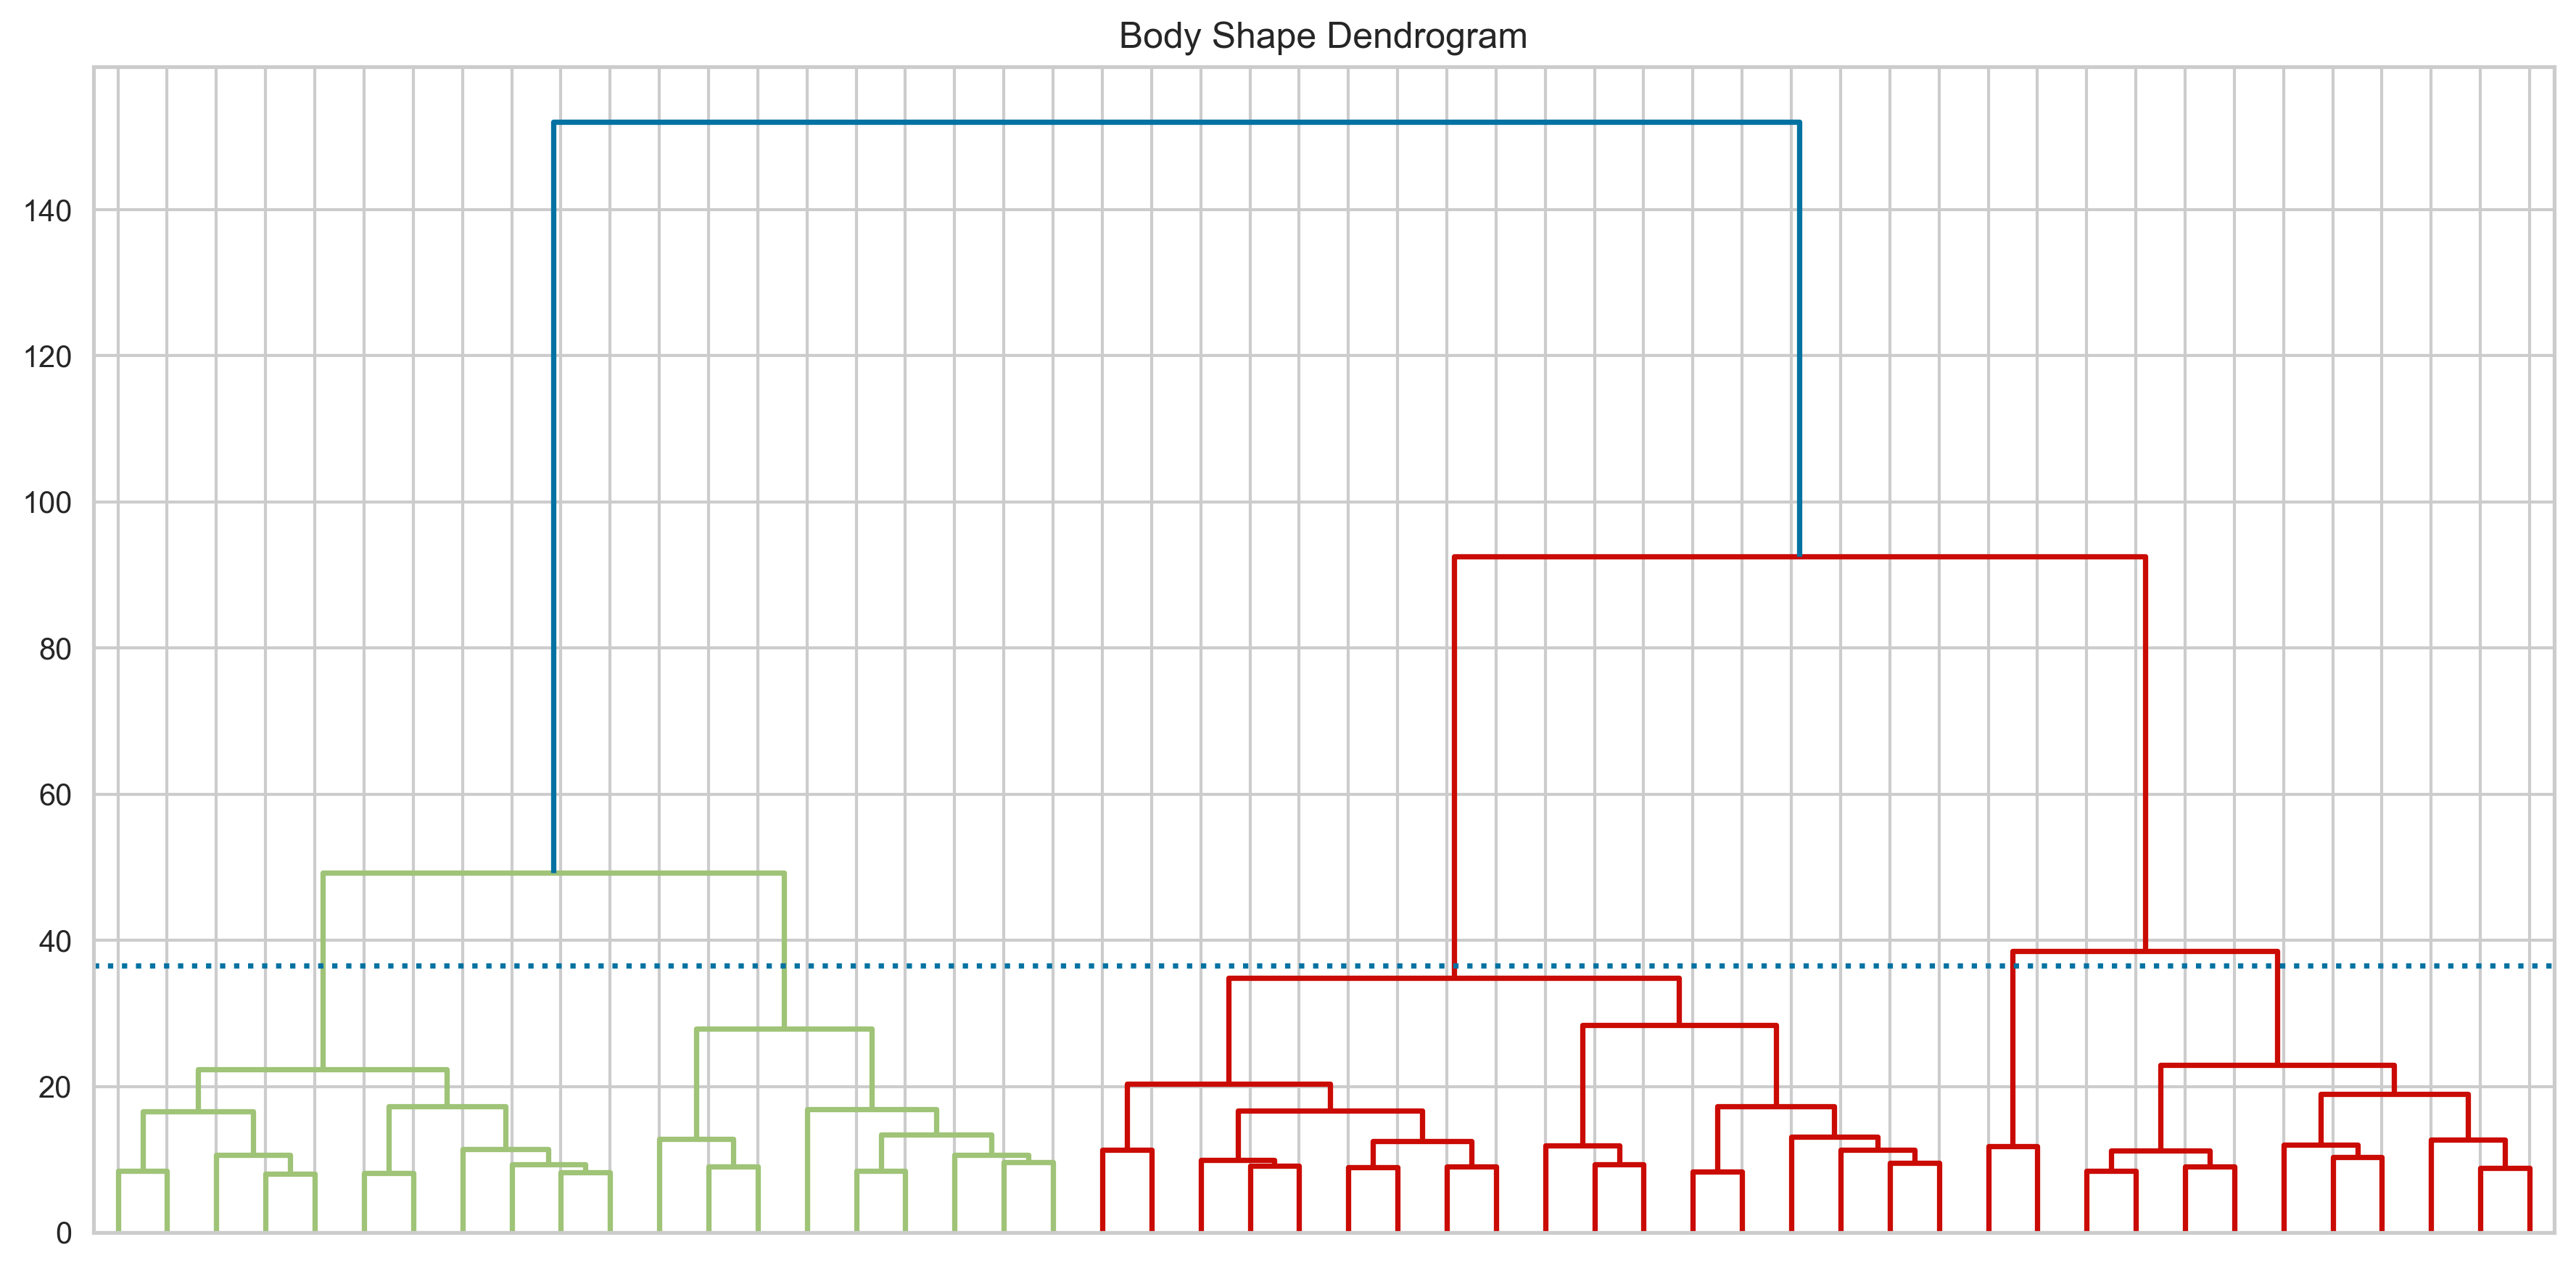
\includegraphics[width=0.95\textwidth]{../Images/FDendrogram.png}
\end{frame}

\begin{frame}{Female Ward's Method Clusters}
	\centering
	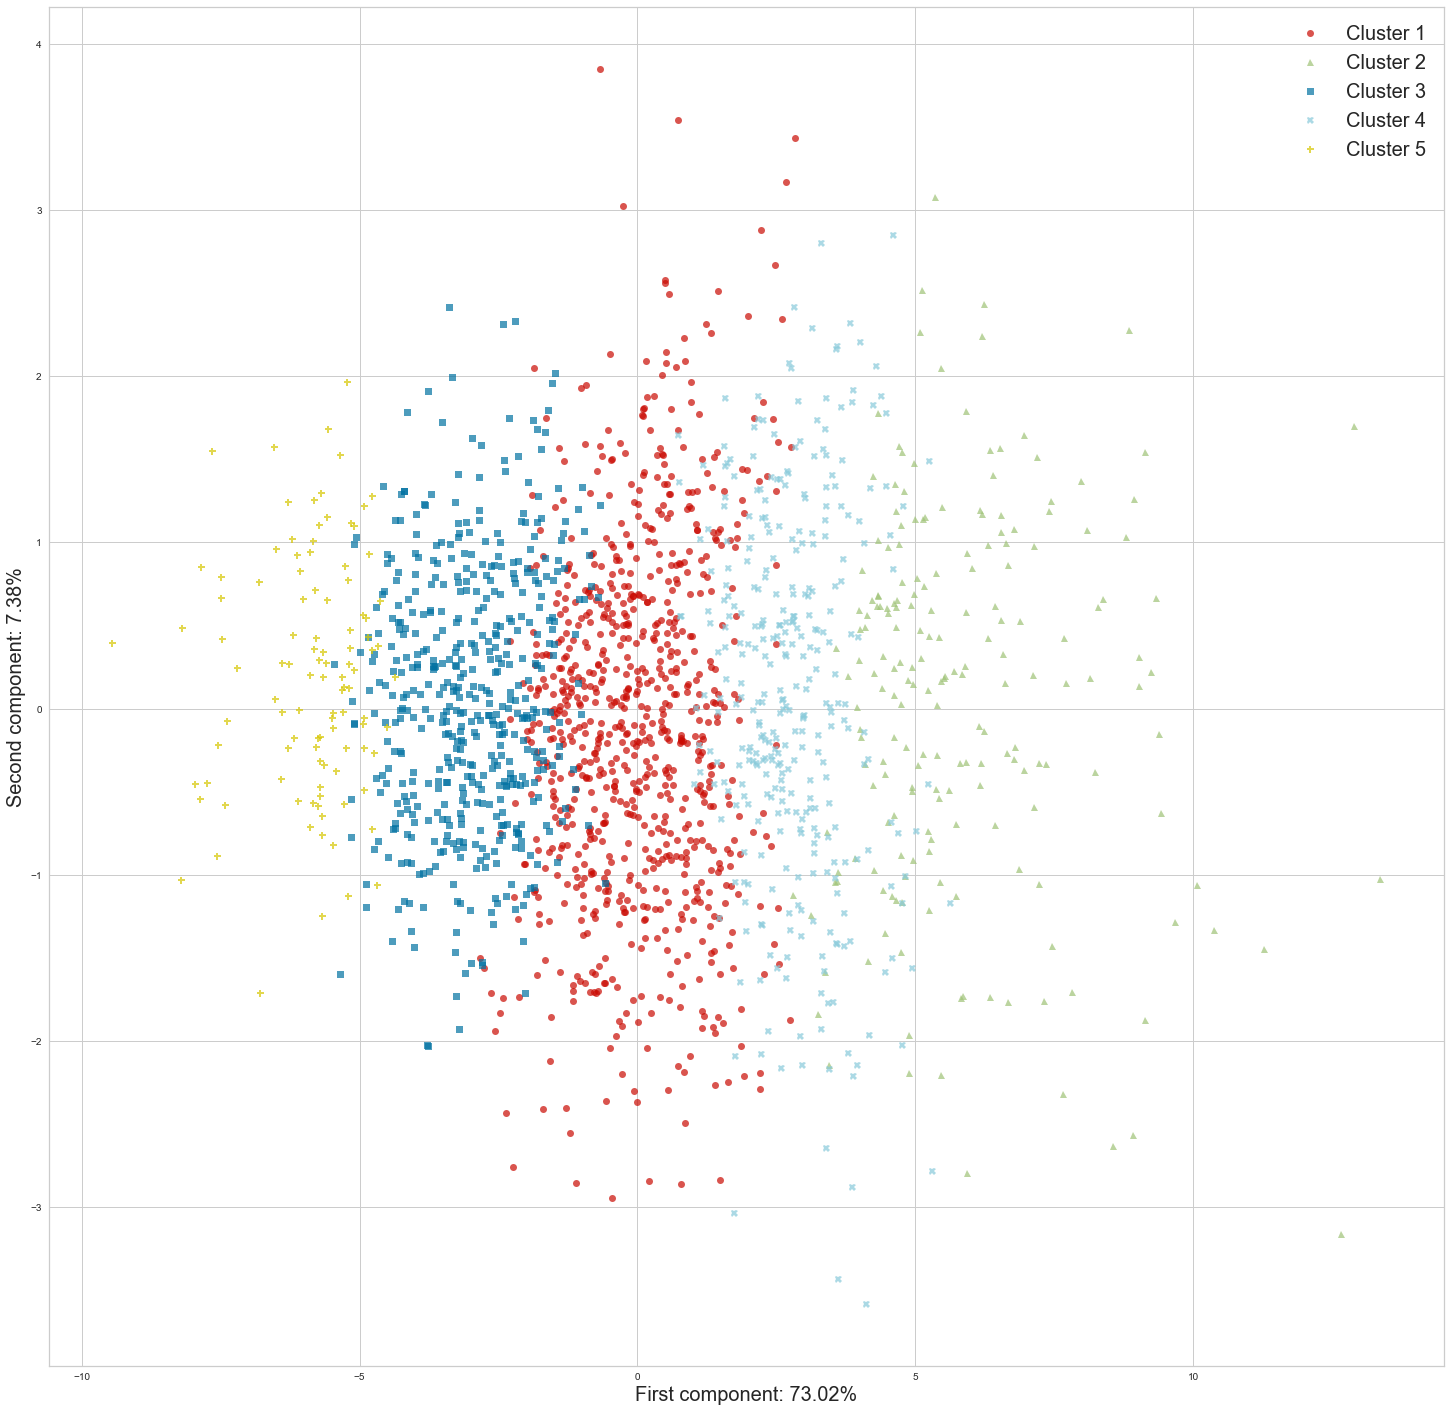
\includegraphics[width=0.675\textwidth]{../Images/FHierProjection.png}
\end{frame}

\subsubsection{Clusters description}
\begin{frame}{Female K-Medoids Medoids}
	\scriptsize
	\centering
	\begin{tabular}{lcccccc}
		\cline{2-7}
		                             & \multicolumn{6}{c}{\textbf{Cluster}}                                                                  \\
		                             & \textbf{1}                           & \textbf{2} & \textbf{3} & \textbf{4} & \textbf{5} & \textbf{6} \\
		\hline\hline
		Bicristal breadth            & 270                                  & 278        & 261        & 260        & 299        & 292        \\
		Buttock circumference        & 970                                  & 1016       & 917        & 1015       & 1136       & 1076       \\
		Buttock depth                & 216                                  & 235        & 193        & 233        & 280        & 251        \\
		Chest breadth                & 258                                  & 281        & 248        & 255        & 295        & 270        \\
		Chest circumference          & 892                                  & 962        & 866        & 906        & 1069       & 998        \\
		Chest depth                  & 227                                  & 253        & 225        & 237        & 287        & 267        \\
		Hip breadth                  & 340                                  & 357        & 322        & 344        & 387        & 366        \\
		Lower thigh circumference    & 395                                  & 402        & 351        & 398        & 443        & 534        \\
		Shoulder circumference       & 993                                  & 1035       & 965        & 1035       & 1075       & 1035       \\
		Thigh circumference          & 588                                  & 623        & 545        & 606        & 702        & 663        \\
		Vertical trunk circumference & 1519                                 & 1581       & 1477       & 1553       & 1639       & 1594       \\
		Waist breadth                & 272                                  & 316        & 268        & 276        & 357        & 324        \\
		Waist circumference          & 807                                  & 886        & 731        & 824        & 1028       & 933        \\
		Waist depth                  & 203                                  & 212        & 176        & 199        & 269        & 232        \\
		\hline
		Height (cm)                  & 160.02                               & 167.64     & 160.02     & 170.18     & 165.10     & 162.56     \\
		Weight (kg)                  & 63.50                                & 65.32      & 56.70      & 70.31      & 81.65      & 73.94      \\
		BMI                          & 24.80                                & 23.24      & 22.14      & 24.28      & 29.95      & 27.98
	\end{tabular}
\end{frame}

\begin{frame}{Female K-Medoids Centroids}
	\scriptsize
	\centering
	\begin{tabular}{lcccccc}
		\cline{2-7}
		                             & \multicolumn{6}{c}{\textbf{Cluster}}                                                                            \\
		                             & \textbf{1}                           & \textbf{2}   & \textbf{3}   & \textbf{4}   & \textbf{5}   & \textbf{6}   \\
		\hline\hline
		Bicristal breadth            & 264.87                               & 279.85       & 250.56       & 257.97       & 304.40       & 285.79       \\
		Buttock circumference        & 971.19                               & 1025.85      & 913.16       & 1015.66      & 1140.41      & 1086.44      \\
		Buttock depth                & 215.91                               & 231.80       & 201.88       & 233.22       & 271.63       & 252.97       \\
		Chest breadth                & 260.40                               & 278.94       & 248.44       & 259.82       & 294.71       & 275.44       \\
		Chest circumference          & 892.16                               & 972.16       & 845.13       & 913.87       & 1084.39      & 995.67       \\
		Chest depth                  & 229.04                               & 254.31       & 215.36       & 239.00       & 290.64       & 263.69       \\
		Hip breadth                  & 338.80                               & 357.38       & 318.61       & 349.07       & 391.98       & 374.09       \\
		Lower thigh circumference    & 383.46                               & 399.40       & 357.00       & 402.33       & 446.39       & 426.38       \\
		Shoulder circumference       & 995.66                               & 1040.72      & 962.36       & 1027.85      & 1102.64      & 1053.20      \\
		Thigh circumference          & 581.25                               & 617.04       & 538.02       & 616.74       & 698.05       & 663.93       \\
		Vertical trunk circumference & 1512.24                              & 1576.08      & 1469.05      & 1542.88      & 1667.78      & 1607.07      \\
		Waist breadth                & 281.69                               & 308.71       & 257.91       & 282.77       & 354.14       & 322.38       \\
		Waist circumference          & 801.46                               & 881.72       & 730.60       & 817.72       & 1031.28      & 932.32       \\
		Waist depth                  & 194.05                               & 215.56       & 177.07       & 202.71       & 265.71       & 234.44       \\
		\hline
		Age                          & 26.64                                & 29.04        & 26.67        & 27.81        & 33.14        & 31.38        \\
		Height (cm)                  & 161.81                               & 164.86       & 160.23       & 164.78       & 168.53       & 166.29       \\
		Weight (kg)                  & 59.84                                & 67.86        & 53.18        & 65.50        & 81.79        & 74.39        \\
		BMI                          & 22.90                                & 25.02        & 20.75        & 24.20        & 29.82        & 27.30        \\
		\hline
		\textit{Count}               & \textit{360}                         & \textit{452} & \textit{299} & \textit{301} & \textit{232} & \textit{342}
	\end{tabular}
\end{frame}

\begin{frame}{Female Hierarchical Medoids}
	\scriptsize
	\centering
	\begin{tabular}{lccccc}
		\cline{2-6}
		                             & \multicolumn{5}{c}{\textbf{Cluster}}                                                     \\
		                             & \textbf{1}                           & \textbf{2} & \textbf{3} & \textbf{4} & \textbf{5} \\
		\hline\hline
		Bicristal breadth            & 271                                  & 299        & 253        & 292        & 232        \\
		Buttock circumference        & 1011                                 & 1136       & 981        & 1076       & 876        \\
		Buttock depth                & 236                                  & 280        & 217        & 251        & 201        \\
		Chest breadth                & 274                                  & 295        & 251        & 270        & 241        \\
		Chest circumference          & 926                                  & 1069       & 872        & 998        & 808        \\
		Chest depth                  & 245                                  & 287        & 221        & 267        & 199        \\
		Hip breadth                  & 346                                  & 387        & 328        & 366        & 306        \\
		Lower thigh circumference    & 408                                  & 443        & 375        & 435        & 360        \\
		Shoulder circumference       & 1013                                 & 1075       & 990        & 1035       & 934        \\
		Thigh circumference          & 635                                  & 702        & 576        & 663        & 510        \\
		Vertical trunk circumference & 1604                                 & 1639       & 1526       & 1594       & 1411       \\
		Waist breadth                & 288                                  & 357        & 273        & 324        & 241        \\
		Waist circumference          & 847                                  & 1028       & 751        & 933        & 694        \\
		Waist depth                  & 213                                  & 269        & 180        & 232        & 168        \\
		\hline
		Height (cm)                  & 162.56                               & 165.10     & 165.10     & 162.56     & 147.32     \\
		Weight (kg)                  & 68.04                                & 81.65      & 58.06      & 73.94      & 46.72      \\
		BMI                          & 24.96                                & 29.95      & 21.30      & 27.98      & 21.53      \\
	\end{tabular}
\end{frame}

\begin{frame}{Female Hierarchical Centroids}
	\scriptsize
	\centering
	\begin{tabular}{lccccc}
		\cline{2-6}
		                             & \multicolumn{5}{c}{\textbf{Cluster}}                                                             \\
		                             & \textbf{1}                           & \textbf{2}   & \textbf{3}   & \textbf{4}   & \textbf{5}   \\
		\hline\hline
		Bicristal breadth            & 272.00                               & 304.44       & 258.05       & 290.10       & 241.75       \\
		Buttock circumference        & 1023.85                              & 1145.92      & 953.31       & 1083.18      & 883.93       \\
		Buttock depth                & 232.58                               & 274.36       & 212.08       & 251.15       & 196.41       \\
		Chest breadth                & 269.94                               & 293.10       & 256.20       & 281.37       & 242.37       \\
		Chest circumference          & 943.96                               & 1084.66      & 878.83       & 1011.03      & 821.18       \\
		Chest depth                  & 246.12                               & 292.01       & 226.07       & 267.25       & 209.18       \\
		Hip breadth                  & 355.12                               & 393.09       & 332.02       & 373.99       & 306.83       \\
		Lower thigh circumference    & 403.12                               & 449.87       & 374.27       & 420.94       & 347.40       \\
		Shoulder circumference       & 1029.85                              & 1107.76      & 989.31       & 1062.31      & 942.58       \\
		Thigh circumference          & 618.78                               & 703.84       & 568.17       & 658.48       & 518.18       \\
		Vertical trunk circumference & 1558.54                              & 1669.85      & 1502.72      & 1615.76      & 1441.26      \\
		Waist breadth                & 298.75                               & 355.29       & 272.37       & 327.45       & 244.24       \\
		Waist circumference          & 856.81                               & 1036.32      & 773.93       & 945.45       & 696.40       \\
		Waist depth                  & 210.79                               & 268.05       & 187.36       & 236.94       & 169.92       \\
		\hline
		Age                          & 28.71                                & 32.90        & 26.76        & 31.36        & 25.73        \\
		Height (cm)                  & 164.20                               & 168.69       & 162,07       & 166,04       & 157.72       \\
		Weight (kg)                  & 66.66                                & 85.16        & 58.00        & 75.04        & 49.88        \\
		BMI                          & 24.78                                & 30.00        & 22.13        & 27.26        & 20.09        \\
		\hline
		\textit{Count}               & \textit{831}                         & \textit{200} & \textit{503} & \textit{347} & \textit{105}
	\end{tabular}
\end{frame}

\subsection{Male Data Set}
\begin{frame}{Male data set}
	\begin{block}{Male data set}
		\centering
		\begin{tabular}{|cccc|c|}
			\hline
			Age   & Height (cm) & Weight (kg) & BMI   & \textit{Count} \\
			\hline
			30.16 & 177.89      & 85.28       & 26.93 & \textit{4082}  \\
			\hline
		\end{tabular}
	\end{block}
\end{frame}

\begin{frame}{Correlation matrix}
	\centering
	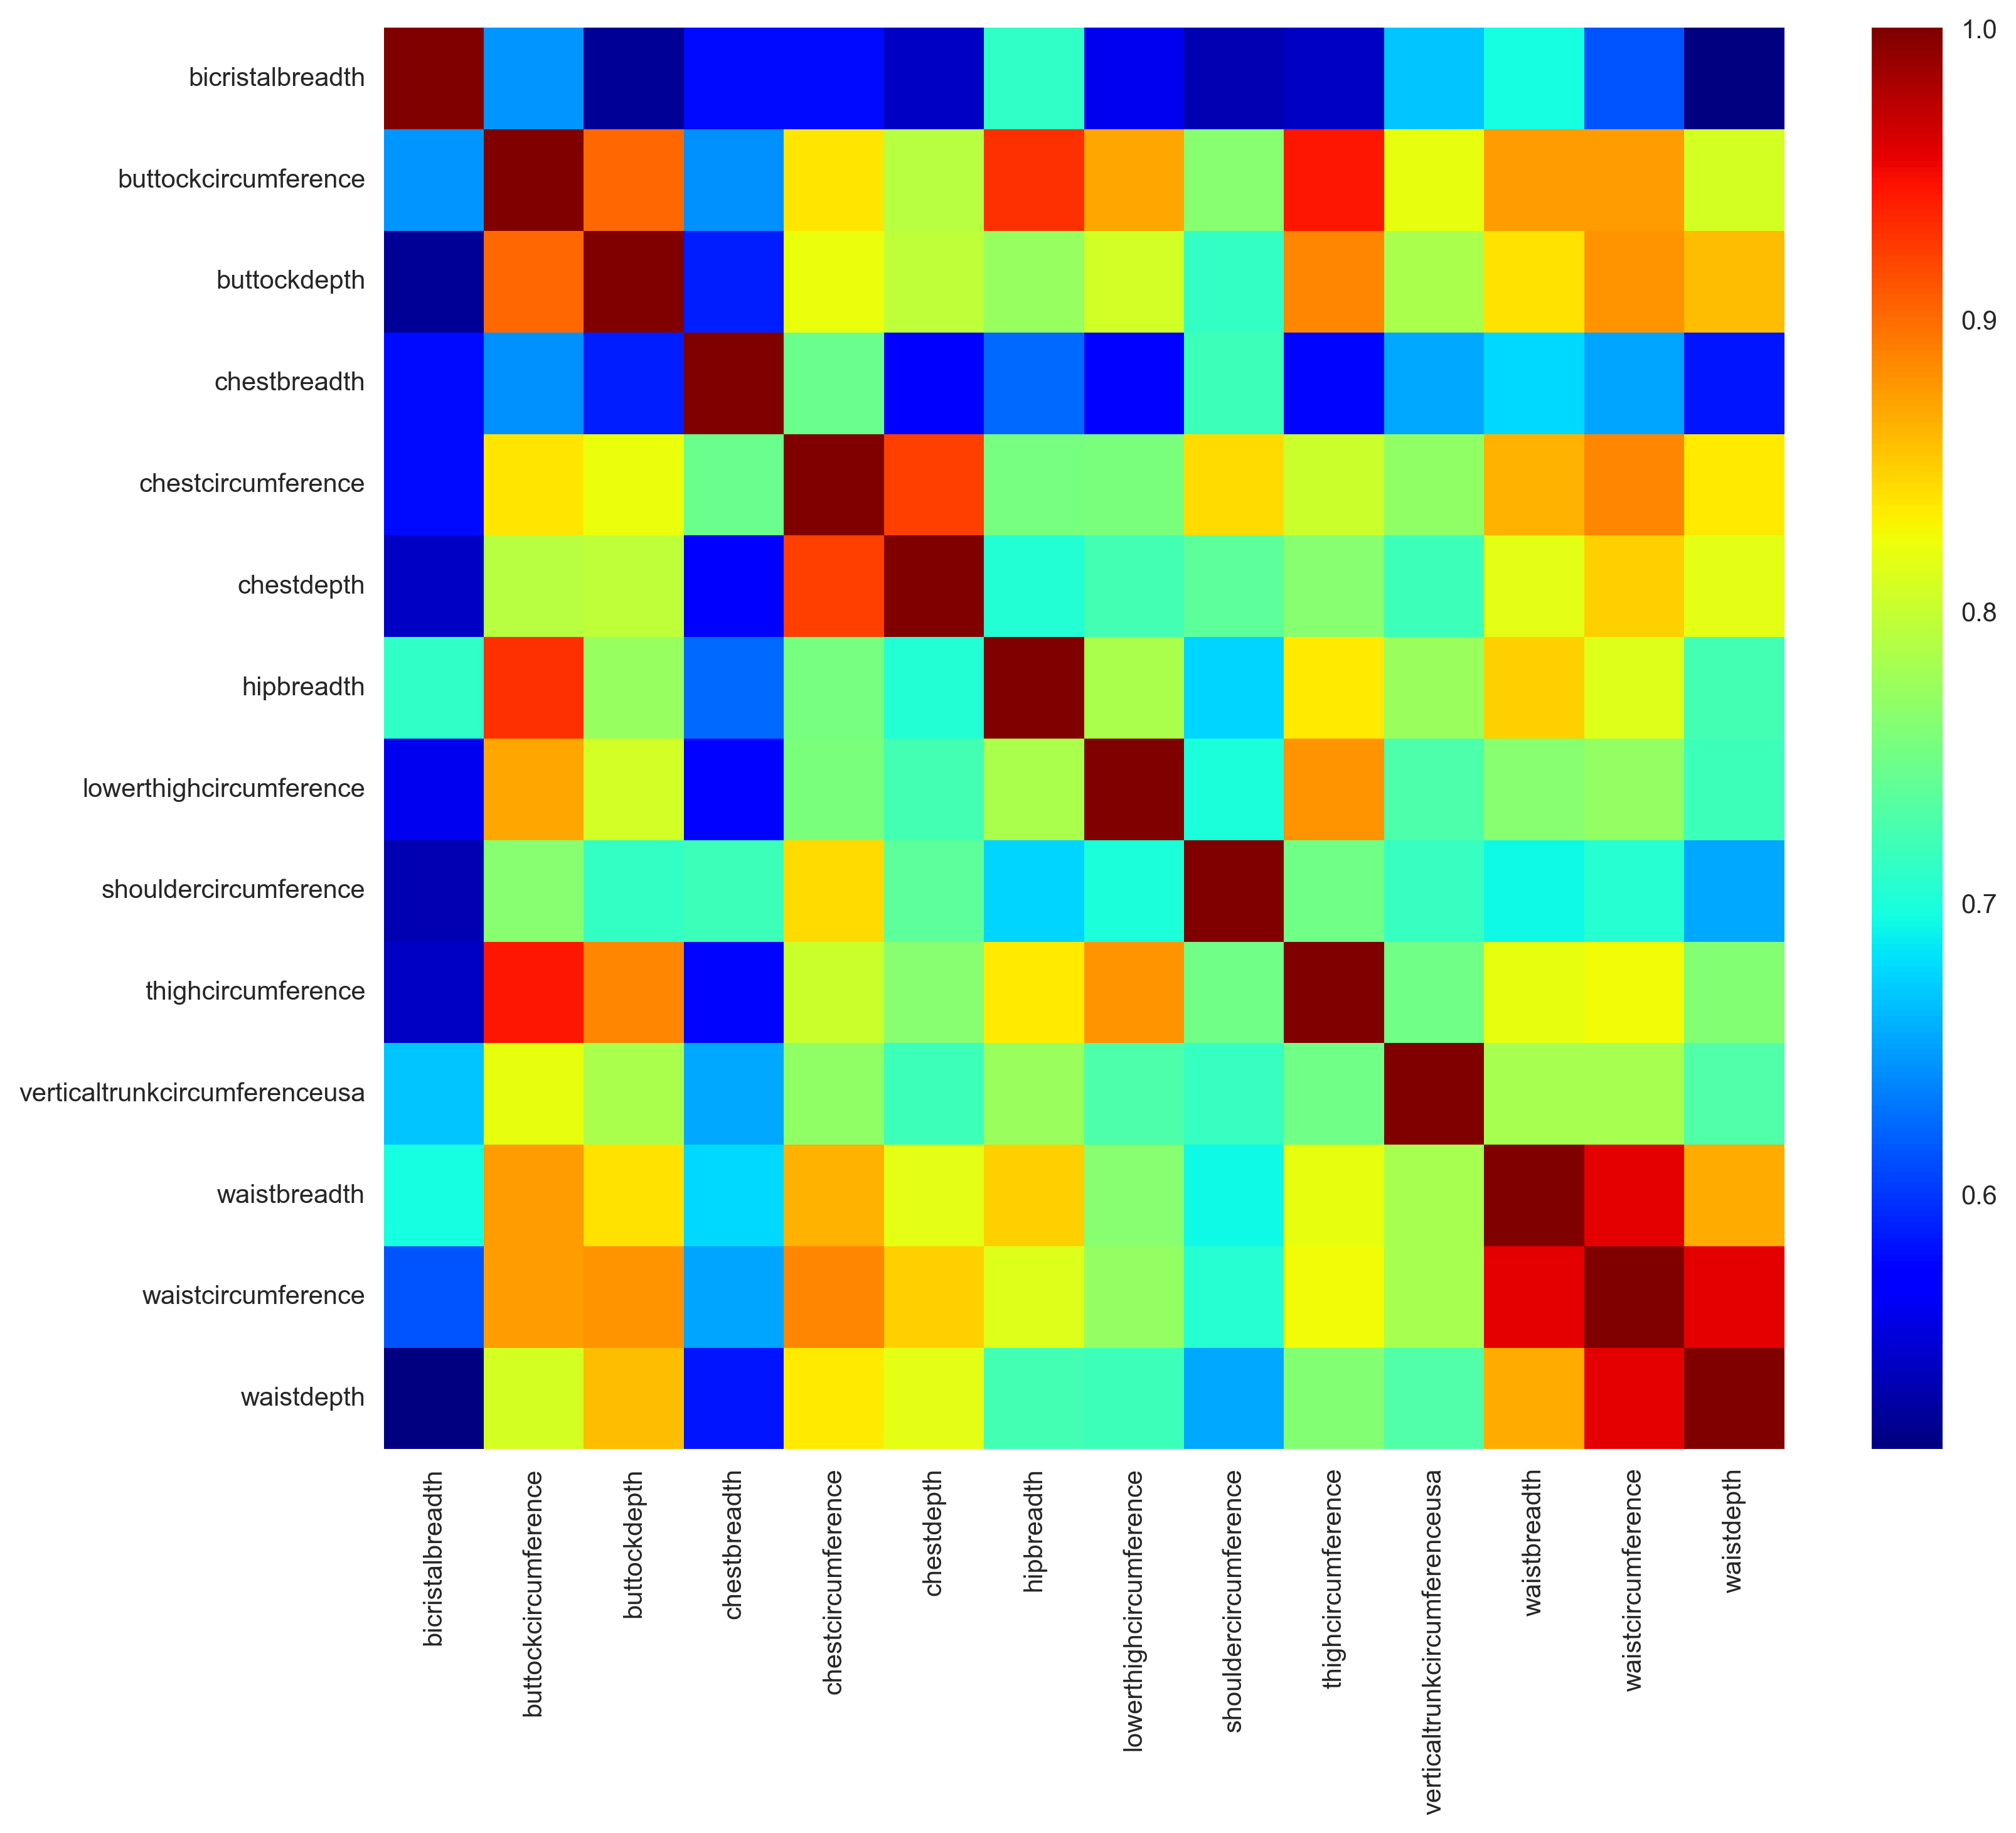
\includegraphics[width=0.7\textwidth]{../Images/MCorr.png}
\end{frame}

\begin{frame}{Elbow method}
	\subsubsection{K-Medoids}
	\begin{minipage}{0.55\textwidth}
		\centering
		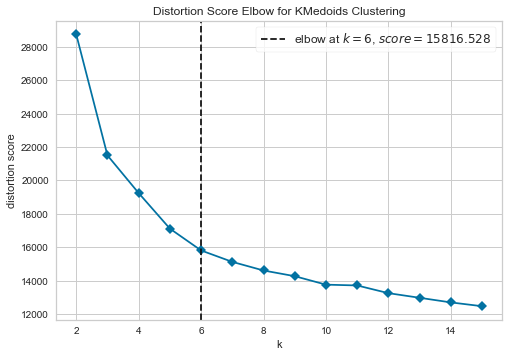
\includegraphics[width=0.8\textwidth]{../Images/MMedoidsElbow.png}
	\end{minipage}
	\begin{minipage}{0.3\textwidth}
		\itshape\scriptsize
		We choose a number of clusters $k=6$ for the K-Medoids.
	\end{minipage}
	\begin{minipage}{0.55\textwidth}
		\centering
		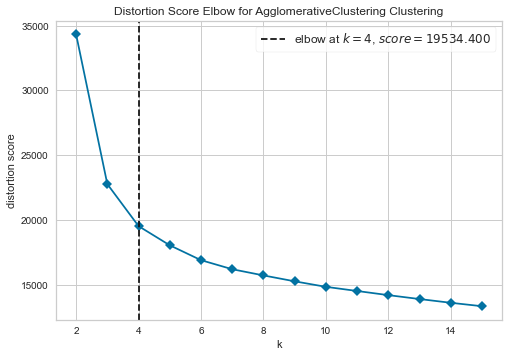
\includegraphics[width=0.8\textwidth]{../Images/MHierElbow.png}
	\end{minipage}
	\begin{minipage}{0.3\textwidth}
		\itshape\scriptsize
		We choose a number of clusters $k=4$ for the Ward's method.
	\end{minipage}
\end{frame}
\subsubsection{Visualisation}
\begin{frame}{K-Medoids Clusters}
	\centering
	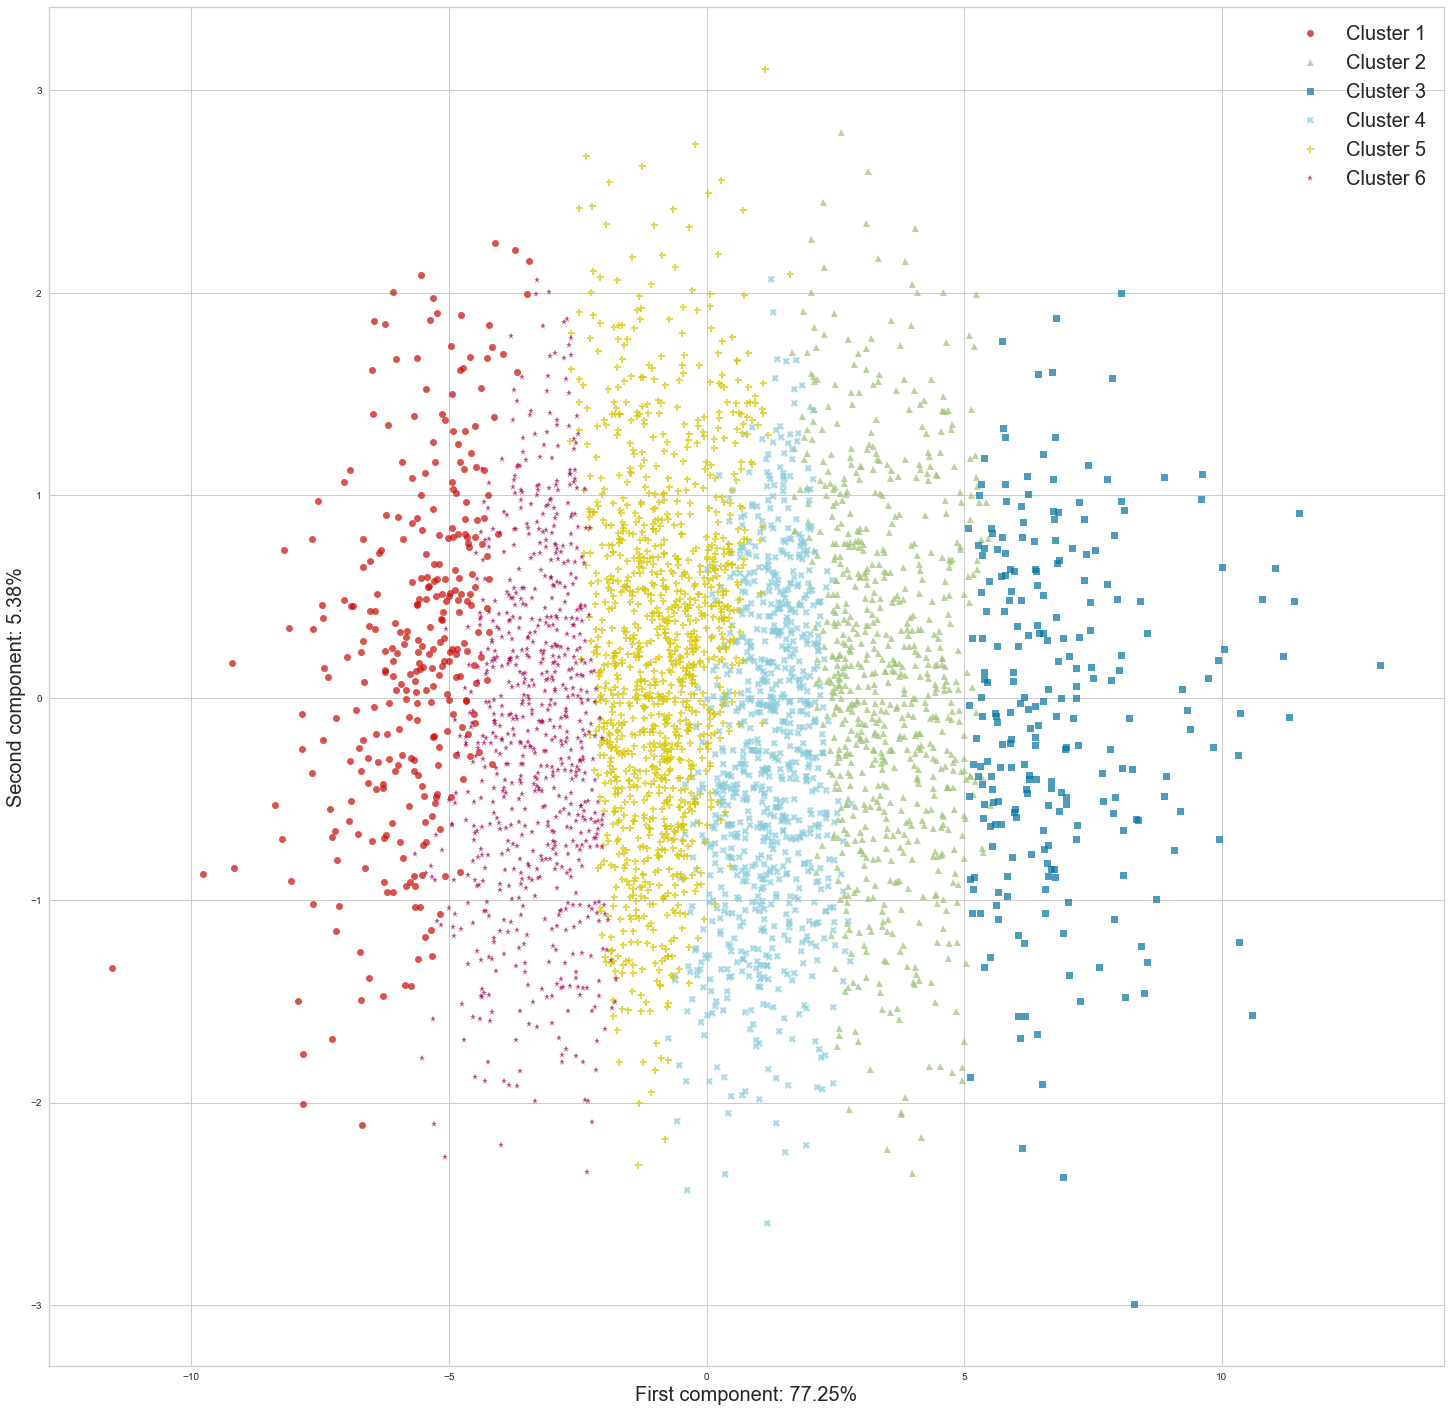
\includegraphics[width=0.675\textwidth]{../Images/MMedoidsProjection.png}
\end{frame}

\begin{frame}{Male Ward's Method Dendrogram}
	\centering
	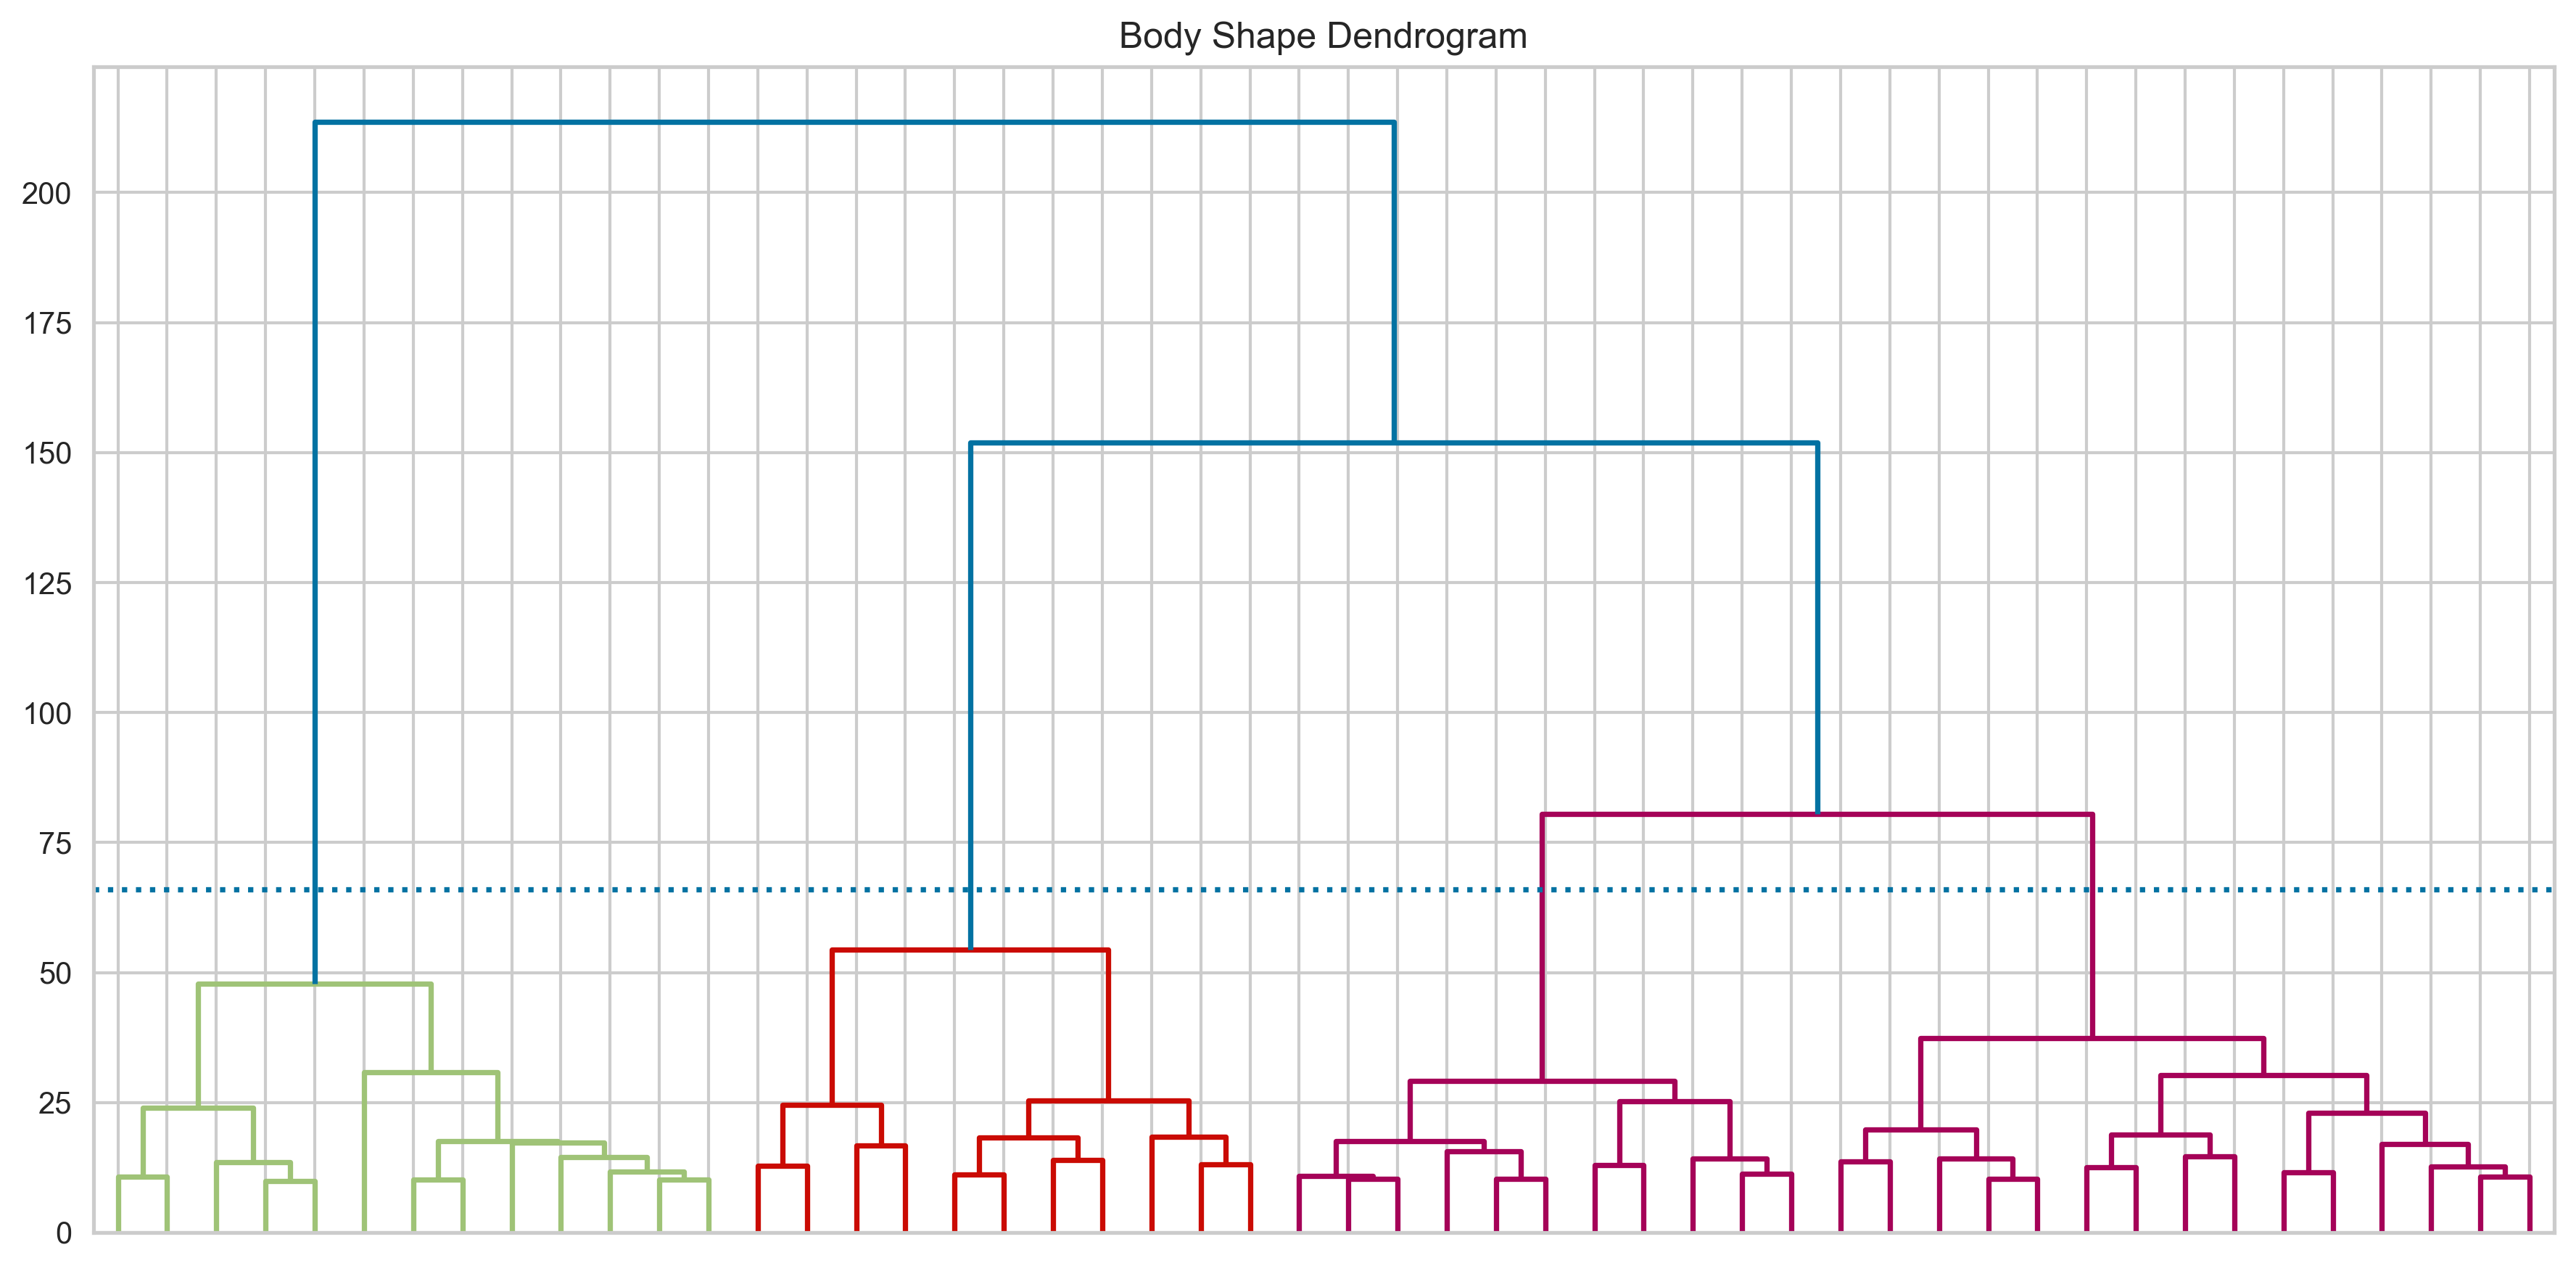
\includegraphics[width=0.95\textwidth]{../Images/MDendrogram.png}
\end{frame}

\begin{frame}{Male Ward's Method Clusters}
	\centering
	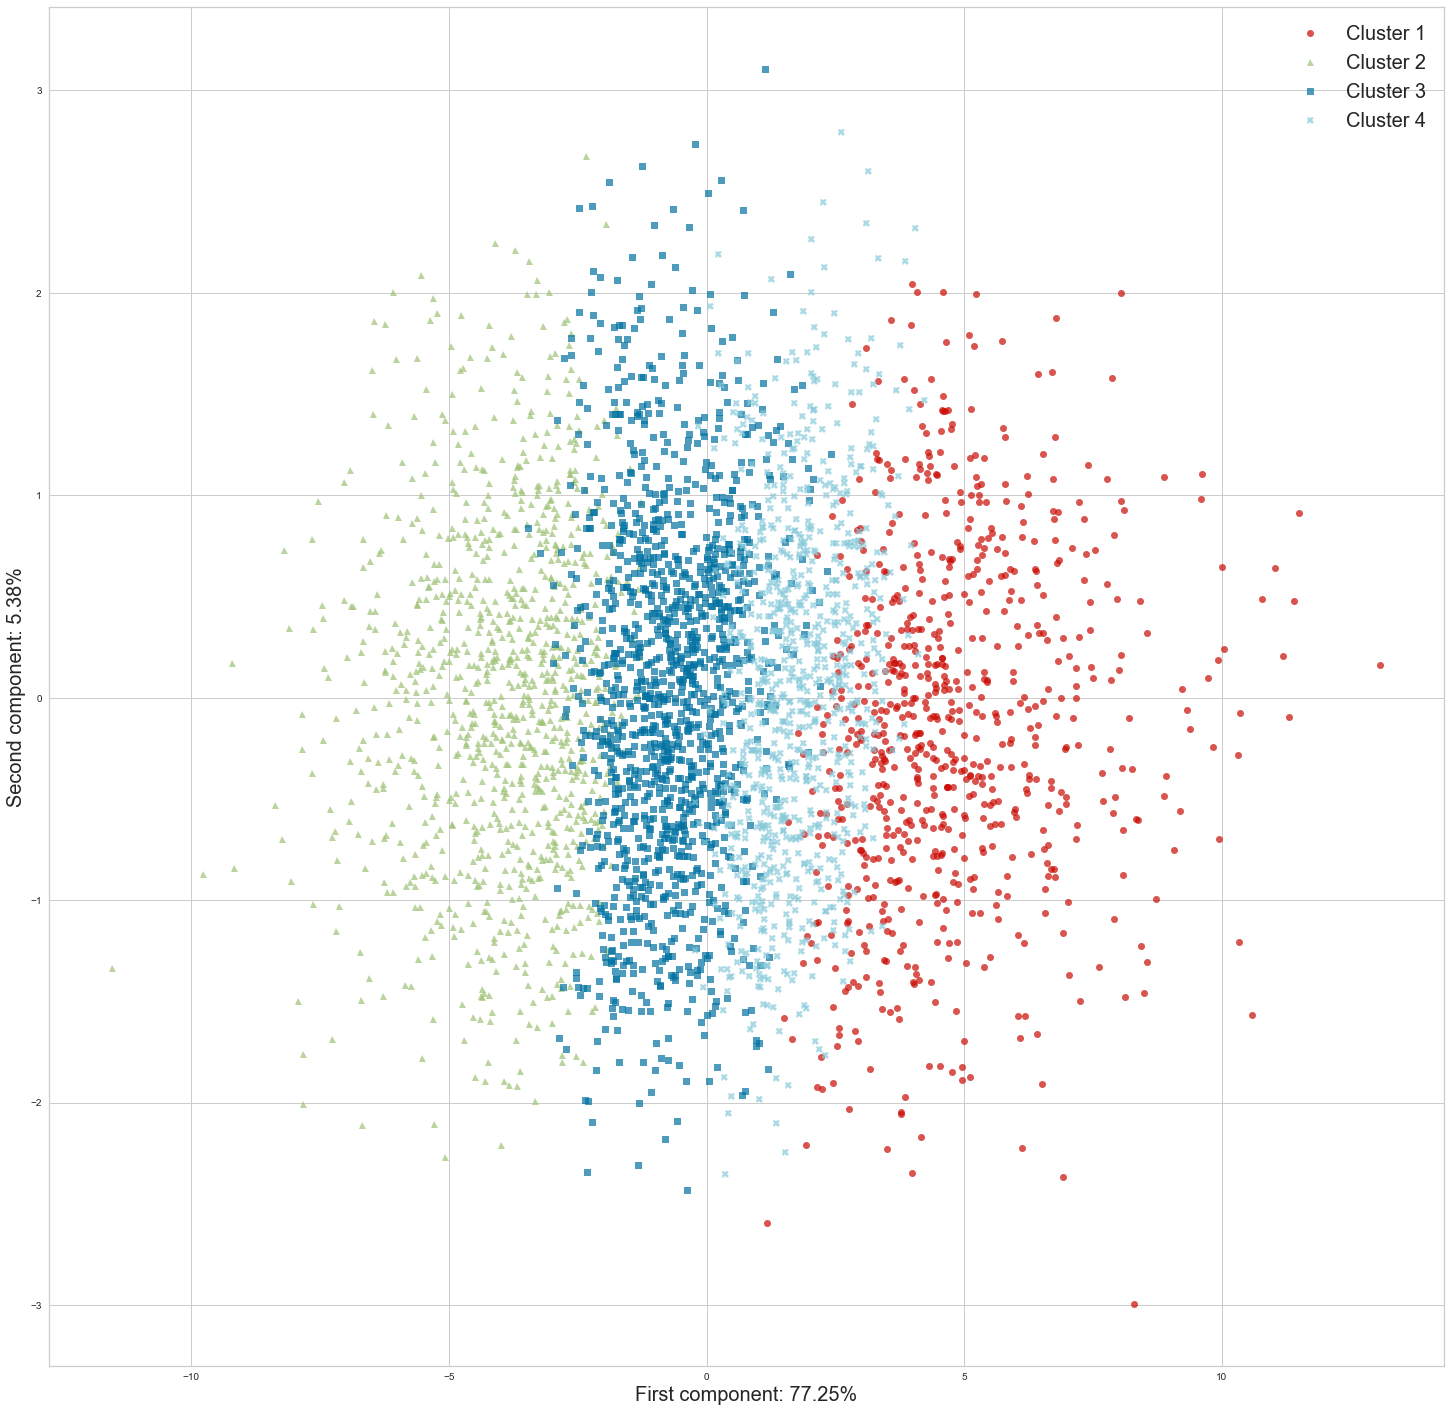
\includegraphics[width=0.675\textwidth]{../Images/MHierProjection.png}
\end{frame}

\subsubsection{Clusters description}
\begin{frame}{Male K-Medoids Medoids}
	\scriptsize
	\centering
	\begin{tabular}{lcccccc}
		\cline{2-7}
		                             & \multicolumn{6}{c}{\textbf{Cluster}}                                                                  \\
		                             & \textbf{1}                           & \textbf{2} & \textbf{3} & \textbf{4} & \textbf{5} & \textbf{6} \\
		\hline\hline
		Bicristal breadth            & 275                                  & 252        & 263        & 293        & 301        & 269        \\
		Buttock circumference        & 1004                                 & 1073       & 916        & 1097       & 1178       & 959        \\
		Buttock depth                & 242                                  & 251        & 214        & 267        & 293        & 220        \\
		Chest breadth                & 288                                  & 298        & 263        & 300        & 316        & 278        \\
		Chest circumference          & 1026                                 & 1100       & 940        & 1145       & 1237       & 996        \\
		Chest depth                  & 241                                  & 266        & 224        & 276        & 304        & 238        \\
		Hip breadth                  & 345                                  & 362        & 317        & 373        & 396        & 331        \\
		Lower thigh circumference    & 403                                  & 437        & 376        & 443        & 460        & 379        \\
		Shoulder circumference       & 1173                                 & 1190       & 1082       & 1245       & 1255       & 1140       \\
		Thigh circumference          & 613                                  & 653        & 553        & 679        & 730        & 587        \\
		Vertical trunk circumference & 1657                                 & 1682       & 1559       & 1742       & 1813       & 1604       \\
		Waist breadth                & 322                                  & 362        & 285        & 367        & 402        & 308        \\
		Waist circumference          & 902                                  & 1012       & 784        & 1078       & 1167       & 860        \\
		Waist depth                  & 220                                  & 255        & 199        & 270        & 306        & 212        \\
		\hline
		Height (cm)                  & 175.26                               & 185.42     & 172.72     & 177.80     & 175.26     & 170.18     \\
		Weight (kg)                  & 79.38                                & 96.62      & 70.31      & 97.52      & 79.38      & 67.13      \\
		BMI                          & 25.84                                & 28.10      & 23.56      & 30.85      & 33.75      & 24.75
	\end{tabular}
\end{frame}

\begin{frame}{Male K-Medoids Centroids}
	\scriptsize
	\centering
	\begin{tabular}{lcccccc}
		\cline{2-7}
		                             & \multicolumn{6}{c}{\textbf{Cluster}}                                                                             \\
		                             & \textbf{1}                           & \textbf{2}   & \textbf{3}   & \textbf{4}   & \textbf{5}    & \textbf{6}   \\
		\hline\hline
		Bicristal breadth            & 258.85                               & 289.87       & 301.60       & 276.16       & 274.10        & 260.88       \\
		Buttock circumference        & 888.46                               & 1097.33      & 1175.34      & 1042.16      & 1002.36       & 947.35       \\
		Buttock depth                & 203.21                               & 270.81       & 297.09       & 256.19       & 238.10        & 222.51       \\
		Chest breadth                & 266.54                               & 304.60       & 315.88       & 292.76       & 287.50        & 284.67       \\
		Chest circumference          & 916.22                               & 1143.49      & 1224.53      & 1096.04      & 1033.34       & 977.17       \\
		Chest depth                  & 212.10                               & 277.48       & 300.32       & 266.28       & 245.60        & 231.38       \\
		Hip breadth                  & 310.12                               & 369.20       & 392.81       & 350.47       & 341.45        & 323.36       \\
		Lower thigh circumference    & 356.46                               & 437.62       & 467.97       & 418.71       & 402.94        & 383.29       \\
		Shoulder circumference       & 1080.04                              & 1235.39      & 1284.64      & 1196.08      & 1166.80       & 1125.71      \\
		Thigh circumference          & 521.68                               & 679.03       & 737.53       & 643.89       & 613.09        & 575.66       \\
		Vertical trunk circumference & 1532.31                              & 1749.64      & 1821.66      & 1686.94      & 1650.50       & 1582.26      \\
		Waist breadth                & 272.79                               & 361.23       & 394.14       & 339.52       & 317.06        & 292.08       \\
		Waist circumference          & 764.56                               & 1051.71      & 1162.59      & 987.48       & 905.36        & 833.12       \\
		Waist depth                  & 188.54                               & 269.77       & 305.78       & 252.28       & 225.12        & 207.64       \\
		\hline
		Age                          & 30.49                                & 32.70        & 25.43        & 32.74        & 31.47         & 26.80        \\
		Height (cm)                  & 174.67                               & 180.69       & 183.11       & 177.06       & 178.46        & 174.84       \\
		Weight (kg)                  & 64.28                                & 98.97        & 113.35       & 89.00        & 81.57         & 72.89        \\
		BMI                          & 26.12                                & 28.63        & 22.18        & 31.20        & 33.79         & 24.04        \\
		\hline
		\textit{Count}               & \textit{1366}                         & \textit{902} & \textit{593} & \textit{528} & \textit{218} & \textit{475}
	\end{tabular}
\end{frame}

\begin{frame}{Male Hierarchical Medoids}
	\scriptsize
	\centering
	\begin{tabular}{lcccc}
		\cline{2-5}
		                             & \multicolumn{4}{c}{\textbf{Cluster}}                                        \\
		                             & \textbf{1}                           & \textbf{2} & \textbf{3} & \textbf{4} \\
		\hline\hline
		Bicristal breadth            & 288                                  & 261        & 275        & 282        \\
		Buttock circumference        & 1134                                 & 954        & 1004       & 1073       \\
		Buttock depth                & 278                                  & 224        & 242        & 251        \\
		Chest breadth                & 304                                  & 275        & 288        & 298        \\
		Chest circumference          & 1118                                 & 968        & 1026       & 1100       \\
		Chest depth                  & 289                                  & 232        & 241        & 266        \\
		Hip breadth                  & 383                                  & 318        & 345        & 362        \\
		Lower thigh circumference    & 459                                  & 382        & 403        & 437        \\
		Shoulder circumference       & 1234                                 & 1112       & 1173       & 1190       \\
		Thigh circumference          & 718                                  & 579        & 613        & 653        \\
		Vertical trunk circumference & 1776                                 & 1561       & 1657       & 1682       \\
		Waist breadth                & 376                                  & 286        & 322        & 362        \\
		Waist circumference          & 1110                                 & 811        & 902        & 1012       \\
		Waist depth                  & 286                                  & 204        & 220        & 255        \\
		\hline
		Height (cm)                  & 177.8                                & 170.18     & 175.26     & 185.42     \\
		Weight (kg)                  & 103.87                               & 67.13      & 79.39      & 96.62      \\
		BMI                          & 32.86                                & 23.18      & 25.84      & 28.10
	\end{tabular}
\end{frame}

\begin{frame}{Male Hierarchical Centroids}
	\scriptsize
	\centering
	\begin{tabular}{lcccc}
		\cline{2-5}
		                             & \multicolumn{4}{c}{\textbf{Cluster}}                                                \\
		                             & \textbf{1}                           & \textbf{2}    & \textbf{3}    & \textbf{4}   \\
		\hline\hline
		Bicristal breadth            & 292.70                               & 261.52        & 271.98        & 282.87       \\
		Buttock circumference        & 1130.19                              & 931.38        & 1003.26       & 1056.97      \\
		Buttock depth                & 282.71                               & 217.15        & 239.82        & 258.46       \\
		Chest breadth                & 306.17                               & 272.56        & 288.38        & 297.21       \\
		Chest circumference          & 1172.70                              & 958.13        & 1045.75       & 1103.14      \\
		Chest depth                  & 286.56                               & 225.26        & 249.70        & 266.93       \\
		Hip breadth                  & 378.40                               & 320.13        & 340.47        & 357.01       \\
		Lower thigh circumference    & 450.08                               & 375.81        & 403.29        & 424.28       \\
		Shoulder circumference       & 1254.00                              & 1113.15       & 1173.93       & 1200.74      \\
		Thigh circumference          & 705.53                               & 560.26        & 615.02        & 650.81       \\
		Vertical trunk circumference & 1779.18                              & 1571.25       & 1648.97       & 1704.96      \\
		Waist breadth                & 374.05                               & 287.00        & 318.79        & 345.34       \\
		Waist circumference          & 1097.06                              & 813.05        & 915.67        & 999.87       \\
		Waist depth                  & 285.36                               & 201.73        & 229.35        & 253.85       \\
		\hline
		Age                          & 32.37                                & 26.04         & 30.49         & 32.70        \\
		Height (cm)                  & 181.10                               & 175.18        & 177.73        & 178.68       \\
		Weight (kg)                  & 104.33                               & 70.31         & 82.31         & 91.23        \\
		BMI                          & 31.95                                & 23.01         & 26.12         & 28.63        \\
		\hline
		\textit{Count}               & \textit{746}                         & \textit{1068} & \textit{1366} & \textit{902}
	\end{tabular}
\end{frame}

\begin{frame}{Conclusion}
	According to the state of the art and the results we have obtained, clustering methods seem to be adapted to the classification of human morphotypes.
	
	Among them, Ward's method associated with a principal component analysis seems to me to be the best.
	
	In the near future, we will continue this study on a database representative of the French population.
\end{frame}

\begin{frame}[allowframebreaks]{Bibliography}
	\bibliography{biblio}
\end{frame}
\end{document}